%%%%%%%%%%%%%%%%%%%%%%%%%%%%%%%%%%%%%%%%%%%%%%%%%%%%%%%%%%%
% EPFL report package, main thesis file
% Goal: provide formatting for theses and project reports
% Author: Mathias Payer <mathias.payer@epfl.ch>
%
% To avoid any implication, this template is released into the
% public domain / CC0, whatever is most convenient for the author
% using this template.
%
%%%%%%%%%%%%%%%%%%%%%%%%%%%%%%%%%%%%%%%%%%%%%%%%%%%%%%%%%%%
\documentclass[a4paper,11pt,oneside,openany]{report}
% Options: MScThesis, BScThesis, MScProject, BScProject
\usepackage[MScThesis,lablogo]{EPFLreport}
\usepackage{xspace}
\usepackage{amsmath}
\usepackage{booktabs}
\usepackage{tikz}
\usepackage{ragged2e}
\usetikzlibrary{positioning,arrows.meta,fit,backgrounds,calc}

% Tighten spacing for compact, continuous layout
\usepackage[compact,nobottomtitles*]{titlesec}
\titleclass{\chapter}{straight}
\titleformat{\chapter}[hang]{\Large\bfseries}{\thechapter.}{0.5em}{}
\titleformat{\section}[hang]{\normalsize\bfseries}{\thesection}{0.5em}{}
\titleformat{\subsection}[runin]{\small\bfseries}{\thesubsection}{0.5em}{}[.]
\titlespacing*{\chapter}{0pt}{0.2\baselineskip}{0.25\baselineskip}
\titlespacing*{\section}{0pt}{0.45\baselineskip}{0.2\baselineskip}
\titlespacing*{\subsection}{0.5em}{0.2\baselineskip}{0.5em}

% Compact lists and floats
\usepackage{enumitem}
\setlist{noitemsep, topsep=0.2em}
\setlist[itemize]{left=0pt}
\floatsep=0.4\baselineskip plus 0.1\baselineskip
\textfloatsep=0.5\baselineskip plus 0.1\baselineskip
\intextsep=0.3\baselineskip plus 0.1\baselineskip

\title{Adaptive Calibration Algorithms\\for Tunable Analog Peripherals}
\author{Khalil M'hirsi}
\date{7 August 2026}
\supervisor{Christophe Constantin}
\adviser{Prof. Mathieu Salzmann}
%\coadviser{Second Adviser}
\expert{Richard Lengagne}
\ackquote{``I struggled for a long time\\
with surviving.\\
And no matter what,\\
you keep finding something\\
to fight for.''\\
--- The Last of Us}
\acknowledgments{%
I would like to express my sincere gratitude to Christophe Constantin, my supervisor at Logitech, for his trust, guidance, and critical perspective throughout this thesis. I am equally thankful to Yael, a close collaborator on this project, whose feedback and thoughtful challenges helped sharpen both the ideas and the direction of the work. I am also deeply grateful to Professor Mathieu Salzmann for his valuable advice, high standards, and steady guidance in ensuring that this thesis remained rigorous and focused.

I would also like to thank Kilian and Frederic for their technical support on the hardware side, and Jozef and Lilou for the many helpful discussions on machine learning and signal processing. I am grateful as well to my teammates Anais and Kevin, to Thomas, and to the broader team at Logitech for the many forms of support that surrounded this work, from technical discussions and thoughtful advice to the practical organization of data-collection sessions and user tests. This thesis would not have taken its final shape without that collective effort.

On a more personal note, I am deeply grateful to my partner, Sophia, for the patience, steadiness, and care she brought throughout a demanding period. Her presence made the difficult moments lighter and the better ones meaningful. I am equally thankful to my close friends Hugo, Christelle, and Maxence, whose encouragement, listening, and honesty helped me keep moving forward when my own perspective narrowed. More broadly, I am grateful to those closest to me who stood by me through a difficult time and helped me carry this work to its conclusion.
}


\begin{document}
\maketitle
\makeacks

\begin{abstract}
Analog peripherals with continuous depth-sensing hardware offer sub-millimetre actuation precision, yet their firmware often relies on static thresholds that ignore per-user biomechanical variance and degrade under neuromotor fatigue. This thesis addresses that gap by designing an end-to-end click-sensitivity recommendation pipeline for Haptic Inductive Trigger System (HITS) devices, using telemetry streamed from the mouse in order to recommend personalized Actuation Level (AL) and Rapid Trigger (RT) settings. The system makes three contributions: (1) a supervised labeling workflow that starts from human-labeled click boundaries and progressively accelerates subsequent labeling through model-assisted iteration; (2) a four-class temporal intent-detection model---supporting Random Forest, Gradient Boosted Trees, and a dilated residual fully-convolutional network---that combines digital signal preprocessing, class-imbalance-aware sample selection, and context-rich features to identify make-onset, click-hold, and break-onset phases from high-frequency telemetry; and (3) a joint CMA-ES optimizer that simulates the firmware click state machine frame-by-frame and finds Pareto-optimal (AL, RT) configurations that reduce actuation latency while maximizing click reliability through explicit constraints on missed clicks and unintended actuations. Together, these components form a practical recommendation workflow from raw HITS telemetry to interpretable parameter recommendations for click sensitivity tuning.
\end{abstract}

\clearpage

\maketoc

% Configure paragraph breaking for two-column mode
% TeX parameters to reduce overfull lines by prioritizing line breaks over tight spacing
\tolerance=2000           % Allow looser justification (default 200, strict)
\emergencystretch=1.5em   % Extra horizontal space when no good break point exists
\hyphenpenalty=50         % Encourage hyphenation over tight spacing

\twocolumn

%%%%%%%%%%%%%%%%%%%%%%
\chapter{Introduction}
%%%%%%%%%%%%%%%%%%%%%%

Human-Computer Interaction (HCI) in high-performance computing and competitive esports places stringent demands on input peripherals. In environments where users execute several hundred Actions Per Minute (APM), actuation latency and threshold stability can affect both task performance and musculoskeletal load~\cite{esports_tendinopathy, wrist_fatigue_genre_2025}.

\section{The Evolution of Continuous Sensing Hardware}
Peripheral hardware has shifted from binary mechanical switches toward continuous sensing interfaces. In HCI, threshold selection and activation logic have long been recognized as key determinants of usability and speed \cite{touchpad_comparison, impact2018}. Recent Hall-effect and inductive devices expose depth-dependent actuation and reset behavior to firmware, including Rapid Trigger mechanisms for dynamic re-actuation \cite{wooting_rapid_trigger, pcgamer_hall_effect, drone_rapid_trigger}. Commercial systems such as HITS further combine inductive sensing with configurable haptic feedback \cite{logitech_superstrike_2026, logitech_hits_patent, fox_superstrike_2026, techradar_superstrike_2026}. Collectively, these developments increase control resolution but also increase dependence on well-calibrated software thresholds \cite{dynamic_keyboard, magnetic_tuning, attackshark_taphold}.

\section{The Limitations of Static Actuation Thresholds}
Despite these hardware leaps, the software interpreting this data remains limited. Current analog peripherals rely on static firmware thresholds that are agnostic to human biomechanical variance. Players exhibit unique control signatures, including micro-hesitations and varying velocity curves, which often clash with rigid hardware logic~\cite{impact2018}. When static thresholds are set too aggressively, they fail to filter out physiological noise; when set too conservatively, they introduce unnecessary mechanical pre-travel. This friction results in sub-optimal latency or a high frequency of unintended actuations during high-stress scenarios~\cite{touchpad_comparison, dynamic_keyboard}.

\section{Neuromotor Fatigue and Performance Decay}
These hardware trends also intersect with user health. Higher APM in esports has been associated with repetitive strain injuries and tendinopathies \cite{esports_tendinopathy, difrancisco2019managing, 1hp_esports_ergonomics}. Biomechanical studies report distinct fatigue patterns for keyboard and mouse interaction \cite{fatigue_flexor}, and repetitive clicking can degrade aiming accuracy while increasing forearm muscle load \cite{clicking_fatigue_ergonomics_2024}. High-APM genres are linked to elevated kinematic demand on wrist extensors \cite{wrist_fatigue_genre_2025}, with measurable neuromotor adaptation during fatiguing tasks \cite{heimhofer2024finger}. These findings motivate adaptive calibration that maintains responsiveness while reducing unintended actuation under fatigue.


\section{Toward Adaptive Intent Detection}
One longer-term direction is intent inference before full mechanical actuation. Prior work on surface electromyography (sEMG) and embedded TinyML suggests this is technically plausible~\cite{reactemg, lda_emg, tinyml_mcu_inference, singh2023edge}. However, this thesis focuses on a narrower and directly evaluable scope: offline calibration from depth telemetry already produced by the peripheral. On-device inference is treated as future work (Section~\ref{sec:conclusion-fw}).

\section{Thesis and Contributions}
The central hypothesis of this thesis is that per-user variation in click telemetry is structured enough to support automatic labeling, statistical modeling, and parameter optimization beyond static default settings. The contributions are:
\begin{itemize}
    \item A programmatic labeling pipeline for analog HID click intent that derives
          frame-level \texttt{MAKE\_ONSET}, \texttt{CLICK\_HOLD}, and \texttt{BREAK\_ONSET}
          annotations from raw depth telemetry without manual annotation, using a
          geometric heuristic as a weak supervision source.
    \item A four-class temporal sequence classifier with two model paths: a shallow
          path (Random Forest, Gradient Boosted Trees) operating on hand-crafted
          sliding-window features for sub-second per-session training, and a deep path
          (dilated residual FCN, CRF decoder) operating on raw telemetry with a
          $\pm$1530\,ms learned receptive field.
    \item A joint CMA-ES optimizer that simulates the peripheral firmware's Rapid
          Trigger state machine and finds Pareto-optimal (AL, RT) configurations,
          replacing manual threshold tuning with a data-driven trade-off curve.
\end{itemize}

%%%%%%%%%%%%%%%%%%%%%%
\chapter{Background}
%%%%%%%%%%%%%%%%%%%%%%

To understand the design and implementation of an adaptive actuation system, it is necessary to establish the technical foundations of continuous sensing hardware, the mathematical logic of modern trigger parameters, and the biomechanical constraints of the human hand.

\section{Continuous Depth-Sensing Mechanisms}

Traditional mechanical switches operate on a binary principle: a circuit is either open or closed based on a physical contact point. In contrast, continuous depth-sensing switches measure the absolute position of the stem throughout its entire travel distance.

\subsection{Hall-Effect and Magnetic Sensing}
Hall-effect sensors utilize a permanent magnet attached to the switch stem and a sensor on the Printed Circuit Board (PCB). As the magnet approaches the sensor, the Hall voltage varies proportionally to the magnetic field strength~\cite{wooting_rapid_trigger, pcgamer_hall_effect}. This allows the firmware to map voltage levels to precise displacement values in millimeters. This technology eliminated "debounce" delay-the physical vibrations of metal leaves-allowing for near-instantaneous signal processing.

\subsection{Haptic Inductive Trigger System (HITS)}
Refined in the 2026 Logitech SUPERSTRIKE series, the Haptic Inductive Trigger System (HITS) replaces magnets with an inductive coil architecture~\cite{logitech_hits_patent, techradar_superstrike_2026}. By measuring changes in electromagnetic induction caused by the proximity of a metallic puck within the trigger, HITS provides higher resolution and lower susceptibility to external magnetic interference compared to Hall-effect sensors. Furthermore, HITS integrates localized haptic motors to simulate tactile "bumps" or "clicks" at software-defined depths, decoupling the physical feel of the switch from its electrical actuation point~\cite{fox_superstrike_2026}.

\section{Control Parameters: AL and RT}

The transition to continuous sensing introduced two primary variables that define the "feel" and speed of an input device.

\subsection{Actuation Level (AL)}
The Actuation Level (AL) is the specific depth ($d$) at which a "key down" event is registered. In traditional switches, this is fixed (e.g., 2.0mm). In analog systems, AL is a variable $d_{act} \in [0.1, 4.0]$mm. Lowering $d_{act}$ reduces mechanical pre-travel, allowing for faster response times, but increases the risk of accidental actuations caused by resting finger weight.

\subsection{Rapid Trigger (RT)}
Rapid Trigger (RT) eliminates the fixed reset point found in mechanical switches. In a standard switch, the key must travel back up past a specific "reset point" before it can be pressed again. RT logic instead monitors the direction of travel. As soon as the stem moves upward by a specific threshold ($\Delta_{up}$), the input resets. Conversely, as soon as it moves back down by $\Delta_{down}$, it reactuates~\cite{wooting_rapid_trigger, drone_rapid_trigger}. This allows for hyper-fast "spamming" of inputs, which is critical in high-APM genres.

\section{Biomechanical Variance and Neuromotor Fatigue}

The efficiency of AL and RT is limited by the physiological state of the user. Human motor control is subject to "signal-dependent noise," where the variance of movement increases with the force or speed of the action.

\subsection{Resting Pressure and Tremors}
Even at rest, users exert varying degrees of force on a peripheral. Factors such as cognitive stress or caffeine intake can cause micro-tremors-high-frequency, low-amplitude oscillations in displacement telemetry~\cite{stress_pressure}. If the AL is set to 0.1mm and the user's tremor amplitude is 0.15mm, the system will register "ghost" inputs.

\subsection{Neuromotor Fatigue Signatures}
Extended sessions lead to fatigue in the \textit{flexor digitorum superficialis} and \textit{extensor digitorum} muscles~\cite{fatigue_flexor, clicking_fatigue_ergonomics_2024}. Fatigue manifests in two measurable telemetry changes:
\begin{enumerate}
    \item \textbf{Velocity Decay:} The "snap-back" velocity (the speed at which a finger releases a key) decreases as the extensor muscles tire~\cite{tholl_wrist_fatigue_2025}.
    \item \textbf{Resting Weight Shift:} As the flexor muscles lose tonicity, the resting weight of the finger often increases, leading to deeper "resting" displacement in the analog sensor~\cite{heimhofer2024finger, 1hp_esports_ergonomics}.
\end{enumerate}

\section{On-Device Inference and TinyML (Scope Context)}

This thesis does not implement or evaluate on-device inference, but brief context is included to position future deployment constraints. Continuous telemetry at high polling rates imposes tight latency budgets that are difficult to satisfy through host-side software alone because of USB polling and OS scheduling behavior~\cite{monaco_sok_2018}. Recent peripheral MCUs, including RISC-V-class devices, are increasingly capable of quantized inference~\cite{tinyml_mcu_inference, tinyml_edge_2025, singh2023edge}. In principle, INT8 models could support pre-report filtering under sub-millisecond deadlines; in practice, validating this claim requires firmware-level access and hardware-in-the-loop measurement, which are out of scope for the present study.

\section{Signal Processing and Optimisation Foundations}
\label{sec:bg-methods}

The adaptive calibration pipeline draws on several established signal processing and machine learning methods. This section describes their mathematical properties; their problem-specific justifications appear in the Design chapter.

\subsection{Savitzky-Golay Smoothing}
Savitzky-Golay (SG) filtering fits a polynomial of degree $p$ to each sliding window of $W$ samples in a least-squares sense and evaluates the polynomial at the window centre~\cite{savitzky_golay_1964}. Because the convolution coefficients are precomputed from the normal equations, the runtime cost is $O(n)$ regardless of window width, identical to a moving average. Crucially, the polynomial fit exactly reproduces moments up to degree $p$, so peak positions and edge inflection points in the signal are not distorted—a property absent from symmetric Gaussian or box filters, which both shift extrema toward the window centre.

\subsection{Hermite Cubic Interpolation: Akima and Makima}
Akima interpolation constructs a piecewise cubic Hermite spline whose tangent at each knot is a weighted average of the four adjacent finite differences, with weights inversely proportional to the absolute difference between consecutive slopes~\cite{akima_1970}. This weighting isolates the tangent estimate from outlier slopes: a single anomalous interval does not propagate ringing across the spline, unlike a natural cubic spline whose tangents are coupled globally. Akima does not enforce monotonicity, so it can represent non-monotone smooth curves. Modified Akima (Makima) adds a half-mean-slope regularisation term to the weight formula, preventing zero-weight degeneracy when two adjacent slopes are equal and opposite—a degenerate case that arises frequently in quantized sensor signals.

\subsection{Covariance Matrix Adaptation Evolution Strategy}
CMA-ES is a derivative-free evolutionary optimiser for continuous search spaces~\cite{hansen_cma_2016}. It maintains a multivariate Gaussian distribution over candidate solutions and, at each generation, moves the distribution mean toward the best-performing candidates and adapts the full covariance matrix to reflect the local curvature of the objective landscape. This covariance adaptation lets the algorithm exploit correlations between parameters and navigate elongated, ill-conditioned valleys that cause gradient-free methods with diagonal step sizes (e.g.\ Nelder-Mead or coordinate descent) to stall. CMA-ES converges in $O(n^2)$ function evaluations for an $n$-dimensional problem, far fewer than the $O(N^n)$ evaluations required by grid search over a width-$N$ grid.

\subsection{Ensemble Methods: Random Forests and Gradient Boosting}
A Random Forest~\cite{breiman_rf_2001} builds an ensemble of decision trees, each trained on a bootstrapped subsample with a random subset of features considered at each split, and averages their posterior class probabilities. The double randomisation decorrelates tree errors, yielding ensemble variance lower than any individual tree without significantly increasing bias. Gradient Boosted Trees~\cite{friedman_gb_2001} instead fit trees sequentially: each tree is trained to correct the pseudo-residual of the current ensemble via gradient descent on a differentiable loss. This staged correction reduces bias relative to a Random Forest, at the cost of longer training time and greater sensitivity to hyperparameter tuning.

\subsection{Bayesian Optimisation and Tree-Structured Parzen Estimators}
Bayesian optimisation builds a probabilistic surrogate model of the objective function and selects the next evaluation point by maximising an acquisition function that balances exploration of uncertain regions against exploitation of known good regions. The Tree-structured Parzen Estimator (TPE)~\cite{bergstra_tpe_2011} implements this by modelling two separate densities over the hyperparameter space: $\ell(x)$ over configurations that produced good results, and $g(x)$ over those that produced poor results. Candidates are drawn from $\ell(x)$ and ranked by the ratio $\ell(x)/g(x)$, concentrating search in regions that distinguish good from bad performance. The Optuna framework~\cite{optuna_akiba_2019} implements TPE with asynchronous evaluation and persistent study storage backed by SQLite.


%%%%%%%%%%%%%%%%
\chapter{Related Work}
%%%%%%%%%%%%%%%%%%%%%%

This chapter surveys prior work across the five domains that the proposed system draws on and contributes to: adaptive threshold methods for HID devices, temporal sequence labeling from biosignals, programmatic labeling and weak supervision, dilated convolutional architectures for sequence modeling, and conditional random fields for sequence labeling.

\section{Adaptive Threshold Methods for HID Devices}

The problem of optimizing actuation parameters for human input devices has a long history in HCI, though prior approaches have relied on fixed heuristics rather than per-user learned models.

Kim et al.~\cite{impact2018} introduced \emph{impact activation}, an alternative actuation scheme for mouse buttons in which a click is registered at the first contact force peak following a rapid finger descent, rather than at a fixed displacement threshold. Their evaluation showed faster reaction times and fewer double-click errors under time pressure. Importantly, impact activation still relies on a single fixed heuristic (the first force peak), making it unsuitable for users with atypical contact dynamics, and it does not adapt to within-session fatigue. This thesis learns thresholds from the user's own recorded telemetry rather than applying a globally fixed policy.

Trewin~\cite{dynamic_keyboard} proposed the \emph{Dynamic Keyboard}, which automatically adjusts keyboard response parameters (minimum press duration, maximum bounce interval) to accommodate users with motor impairments, by observing an initial calibration sequence and adjusting parameters using rule-based adaptation. The Dynamic Keyboard targets binary on/off switch events and adjusts temporal debounce windows; it does not exploit continuous analog depth signals, and its adaptation rules are domain-expert heuristics rather than models trained from user data. The proposed system is complementary in motivation---both aim to reduce unintended actuations---but operates at a different signal level (continuous depth at 1\,kHz vs.\ binary event timing) and uses a data-driven model rather than hand-coded rules.

To the best of our knowledge, peer-reviewed literature has not yet reported a complete learning-based pipeline for automatic joint tuning of Rapid Trigger (RT) and Actuation Level (AL). Current commercial implementations~\cite{wooting_rapid_trigger, logitech_superstrike_2026} primarily expose RT and AL as user-adjusted controls without closed-loop personalization. The joint CMA-ES optimizer in this thesis therefore positions RT/AL tuning as an explicitly optimized per-user objective rather than a manual configuration task.

\section{Temporal Sequence Labeling in Biosignal Processing}

Detecting click intent from continuous depth telemetry is an instance of temporal sequence labeling, a problem that has received substantial attention in the context of richer biosignals.

Surface electromyography (sEMG) is the closest related modality. Wang et al.~\cite{reactemg} presented ReactEMG, which uses masked autoencoder pretraining on sEMG to achieve stable, low-latency intent detection from eight-channel surface electrode recordings. Antuvan and Masia~\cite{lda_emg} applied Linear Discriminant Analysis to simultaneous classification of wrist and finger movements from sEMG, demonstrating real-time throughput on embedded hardware. Both systems operate on multi-channel electrode signals that encode rich neuromuscular information before mechanical actuation occurs; their signal-to-noise advantage over single-sensor depth telemetry is substantial. The proposed system, by contrast, uses only the depth signal already present in the peripheral itself, requiring no additional sensing hardware. This imposes a harder classification problem---depth telemetry cannot observe pre-actuation motor intent---but removes the deployment barrier of wearable electrodes.

Keystroke dynamics literature~\cite{typeformer2022, continuous_keystroke_mdpi} models typing patterns for biometric authentication from binary key event timestamps. TypeFormer~\cite{typeformer2022} applies a Transformer architecture to sequences of inter-key timings and achieves high verification accuracy on mobile devices. These methods treat the keystroke as an atomic event and model the temporal pattern between events; they do not model sub-millisecond intra-click dynamics. The proposed system operates at a finer granularity---frame-level classification at 1\,kHz---which requires a different feature engineering approach and exposes a different class of failure modes (contact-bounce artefacts, quantization noise) absent from binary event streams.

\section{Weak Supervision and Programmatic Labeling}

The geometric auto-labeler introduced in Section~\ref{sec:features} is an instance of the programmatic labeling framework introduced by Ratner et al.\ in Snorkel~\cite{ratner_snorkel_2020}. Snorkel defines \emph{labeling functions}---heuristic rules, distant supervision signals, or domain-expert logic---that each assign noisy labels to unlabeled examples, and combines them via a generative model that learns the accuracy and correlations of each labeling function. The combined label distribution is used as the training signal for a downstream discriminative model.

The geometric auto-labeler in this thesis operates as a single labeling function: a depth-geometry heuristic that assigns \texttt{MAKE\_ONSET}, \texttt{CLICK\_HOLD}, \texttt{BREAK\_ONSET}, and \texttt{BG} labels by backward and forward search from hardware-reported click events. Unlike Snorkel, which combines multiple independent labeling functions and explicitly denoises their disagreements, the proposed system relies on a single labeling function and tasks the ML classifier with learning to correct its known systematic errors (timing bias, plateau ambiguity, missed onsets). Asymmetric soft labels---described in Section~\ref{sec:training}---encode the auto-labeler's directional timing uncertainty into the training signal rather than treating boundary labels as hard observations.

\section{Dilated Convolutions for Sequence Modeling}

The OfflineFCN architecture adapts the dilated causal convolution structure introduced by van den Oord et al.\ in WaveNet~\cite{van_den_oord_wavenet_2016} for raw audio generation. WaveNet stacks dilated causal convolutional layers with exponentially increasing dilation rates to achieve a large receptive field with manageable parameter counts. The dilation schedule $d_i = 2^i$ allows the stack to cover $\sum 2^i$ steps of context with $O(\log N)$ layers rather than the $O(N)$ layers that a fixed-dilation architecture would require.

The OfflineFCN departs from WaveNet in one critical dimension: it uses symmetric (non-causal) padding rather than causal (left-only) padding. This doubles the effective receptive field per layer for the same kernel size, since context is drawn from both directions---enabling the $\pm$1530\,ms receptive field of Equation~\eqref{eq:rf} to be achieved with only 8 blocks. The trade-off is that the resulting model cannot be deployed for streaming inference, since each output depends on future samples. This is appropriate for the offline analysis mode but excludes the model from the on-device path described as future work.

Temporal Convolutional Networks (TCN)~\cite{bai_tcn_2018} present an alternative parameterization of dilated convolutional sequence models for time-series tasks, using causal padding and residual connections similar to the OfflineFCN. TCNs have been shown to match or exceed LSTM performance on a range of sequence labeling tasks with lower training cost. The OfflineFCN's non-causal design is deliberately chosen over a TCN-style causal model because the offline analysis setting places no constraint on causality, and the doubled receptive field provides stronger temporal context for click boundary detection. A causal TCN variant would be the natural architectural choice if on-device streaming inference were required.

\section{Conditional Random Fields for Sequence Labeling}

The CRF output layer follows the formulation of Lafferty, McCallum, and Pereira~\cite{lafferty_crf_2001}, who introduced CRFs as discriminative probabilistic models for segmenting and labeling sequence data. A linear-chain CRF defines a conditional distribution $p(\mathbf{y}|\mathbf{X})$ that decomposes into per-frame emission scores and pairwise transition scores, optimised jointly to maximise the conditional log-likelihood of the label sequence. Viterbi decoding recovers the globally optimal label sequence in $O(T \cdot |\mathcal{Y}|^2)$ time.

CRFs have been widely applied to sequence labeling in natural language processing and to biosignal segmentation. In the proposed system, the key benefit of the CRF over per-frame argmax decoding is constraint enforcement: the learned transition matrix assigns strongly negative scores to physically impossible label transitions such as \texttt{BREAK\_ONSET} immediately following \texttt{BG} (a break without a prior make). Per-frame softmax cannot enforce these structural constraints, leading to fragmented or inverted label sequences under conditions of high class imbalance or low posterior confidence. The CRF wrapper adds this constraint at inference time without modifying the backbone architecture or retraining procedure.


%%%%%%%%%%%%%%%%%%%%
\chapter{Design}
\label{chap:design}
%%%%%%%%%%%%%%%%

The key design contributions of this work are: (1) a Makima superresolution velocity estimator that recovers sub-step motion information from the quantized step120 depth signal, enabling accurate onset timing on 1\,kHz telemetry; (2) a four-class probabilistic intent formulation that decouples make and break detection thresholds, giving independent control over sensitivity at each click boundary; and (3) a joint CMA-ES sweep over the two-dimensional AL/RT parameter space that replaces manual threshold selection with a data-driven Pareto frontier. Prior adaptive-threshold systems for analog HID devices~\cite{impact2018, dynamic_keyboard} apply fixed heuristics independently to each parameter; the joint optimizer here treats the two-dimensional search as a single covariance-adapted problem, exploiting the structural correlation between actuation depth and release sensitivity.

To realize these contributions, the system must solve three tightly coupled problems: faithfully reconstructing the underlying intent signal from noisy, high-rate sensor data; identifying where in that signal a deliberate click begins and ends; and finding AL/RT settings that minimize latency while suppressing false events. This chapter describes the problem-specific reasoning behind each architectural choice; the mathematical properties of the underlying methods are summarised in Section~\ref{sec:bg-methods}.

\section{Design Goals and Constraints}

The system operates in two distinct modes. The \emph{offline analysis} mode is the primary mode of operation: after a gaming session, recorded telemetry is post-processed to detect click boundaries, simulate the RT state machine across a grid of (AL, RT) candidates, and recommend optimal settings. This path has no hard latency constraint beyond user-perceived session-review time (seconds to low tens of seconds). The \emph{on-device inference} mode is the secondary path: a quantized TinyML model resident on the peripheral MCU classifies each telemetry frame as an intended click or physiological noise before the HID report is issued. This path does interpose in the signal chain and must complete within a single polling interval—125\,$\mu$s at 8,000\,Hz, or 1\,ms at the dominant 1,000\,Hz polling rate of modern gaming mice.

\emph{Note: the on-device inference path described here is a design target. The current implementation covers the offline analysis path in full; on-device deployment of a quantized causal model is left as future work (Section~\ref{sec:conclusion-fw}).}

The distinction matters for filter design. Offline components may be zero-phase (non-causal), applying symmetric convolutions over the full recorded session to preserve onset timing without phase lag. On-device components must be causal—each output depends only on current and past samples. The design makes this split explicit: zero-phase Savitzky-Golay smoothing is used for post-hoc analytics and RT simulation, while causal exponential moving averages handle live drift estimation.

A further constraint is personalization. Because no two users share identical biomechanical signatures~\cite{impact2018}, the system avoids globally-fixed thresholds. Every adaptive parameter is fitted per-recording to the individual user's own telemetry.

\section{System Architecture}

The pipeline is structured in four layers, shown in Figure~\ref{fig:arch}. Raw step-depth telemetry is acquired from the peripheral firmware and persisted to a local session store. The \emph{signal processing} layer derives smoothed depth, velocity, acceleration, jerk, and drift channels from the raw data. The \emph{intent detection} layer identifies click boundaries using either a fast geometric onset detector or a trained probabilistic classifier. The \emph{optimization} layer searches the two-dimensional (AL, RT) parameter space using a derivative-free evolutionary optimizer and exposes a Pareto-optimal trade-off curve to the user.

Native C++ daemons handle device I/O, raw frame capture, binary frame decoding, and on-device model execution, communicating with the host application via named pipes. Python services for classifier training, Bayesian hyperparameter search, and parameter optimization run as persistent subprocess workers communicating over an IPC channel. A pool of concurrent optimizer workers enables parallel candidate evaluation; throughput scales linearly with pool size.

\begin{figure}[t]
  \centering
  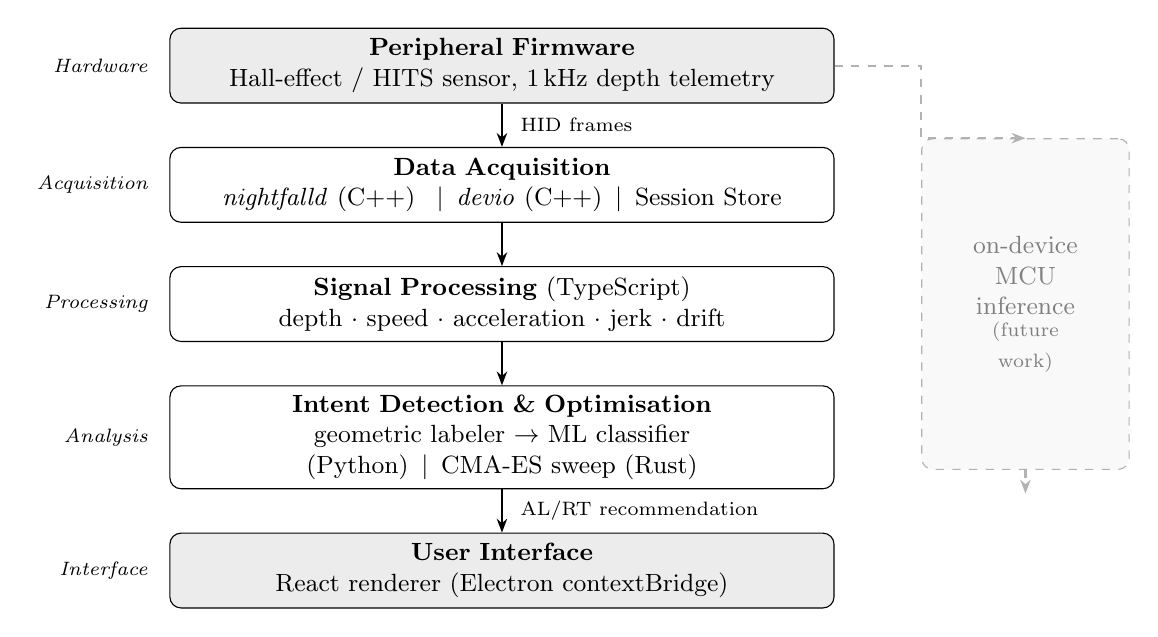
\begin{tikzpicture}[
    font=\small,
    box/.style={draw, rounded corners=4pt, text width=8.2cm,
                minimum height=0.95cm, align=center, fill=white},
    hwbox/.style={draw, rounded corners=4pt, text width=8.2cm,
                  minimum height=0.95cm, align=center, fill=gray!15},
    futurebox/.style={draw=gray!60, dashed, rounded corners=4pt, text width=2.4cm,
                      minimum height=4.2cm, align=center, fill=gray!5, text=gray},
    arr/.style={-{Stealth[length=5pt]}, thick},
    darr/.style={-{Stealth[length=5pt]}, thick, dashed, gray!60},
    node distance=0.55cm,
  ]
    \node[hwbox] (hw)   {\textbf{Peripheral Firmware}\\Hall-effect / HITS sensor, 1\,kHz depth telemetry};
    \node[box,   below=of hw]   (acq)   {\textbf{Data Acquisition}\\
                                          \textit{nightfalld} (C++) \enspace$\vert$\enspace \textit{devio} (C++)\enspace$\vert$\enspace Session Store};
    \node[box,   below=of acq]  (proc)  {\textbf{Signal Processing} (TypeScript)\\
                                          depth $\cdot$ speed $\cdot$ acceleration $\cdot$ jerk $\cdot$ drift};
    \node[box,   below=of proc] (det)   {\textbf{Intent Detection \& Optimisation}\\
                                          geometric labeler $\to$ ML classifier (Python)\enspace$\vert$\enspace CMA-ES sweep (Rust)};
    \node[hwbox, below=of det]  (ui)    {\textbf{User Interface}\\React renderer (Electron contextBridge)};

    \draw[arr] (hw)   -- node[right=3pt, font=\scriptsize] {HID frames} (acq);
    \draw[arr] (acq)  -- (proc);
    \draw[arr] (proc) -- (det);
    \draw[arr] (det)  -- node[right=3pt, font=\scriptsize] {AL/RT recommendation} (ui);

    % On-device future path (dashed, right column)
    \node[futurebox, right=1.1cm of proc] (ondev)
        {on-device\\MCU\\inference\\{\scriptsize (future\\work)}};
    \draw[darr] (hw.east)  -- ++(1.1,0) |- (ondev.north);
    \draw[darr] (ondev.south) -- ++(0,-0.3);

    % Layer label braces
    \node[font=\scriptsize\itshape, left=0.15cm of hw]   {Hardware};
    \node[font=\scriptsize\itshape, left=0.15cm of acq]  {Acquisition};
    \node[font=\scriptsize\itshape, left=0.15cm of proc] {Processing};
    \node[font=\scriptsize\itshape, left=0.15cm of det]  {Analysis};
    \node[font=\scriptsize\itshape, left=0.15cm of ui]   {Interface};
  \end{tikzpicture}
  \caption{Four-layer system architecture. The offline analysis path (solid) post-processes recorded sessions; the on-device inference path (dashed) is a future deployment target for a quantized causal model on the peripheral MCU.}
  \label{fig:arch}
\end{figure}

\begin{figure}[t]
  \centering
  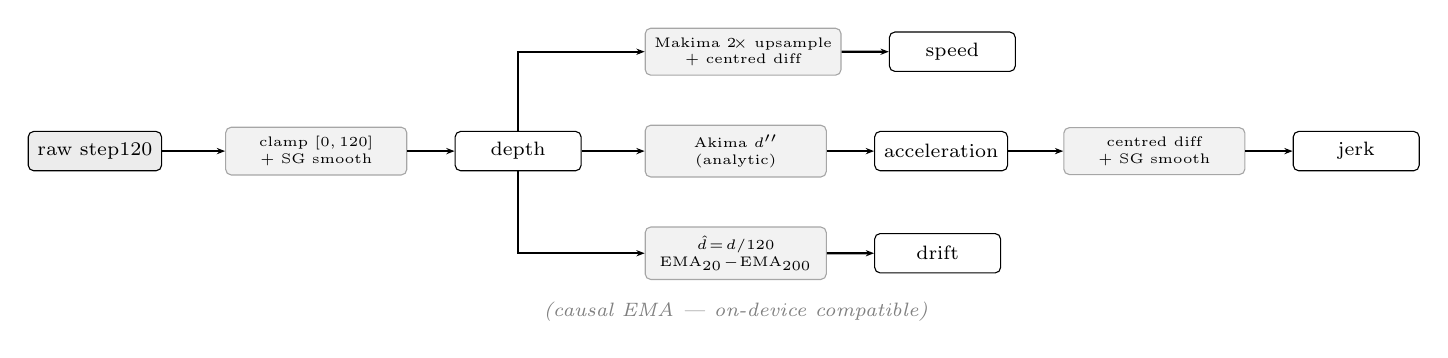
\begin{tikzpicture}[
    font=\small,
    scale=0.85,
    sig/.style={draw, rounded corners=2pt, minimum width=1.6cm, minimum height=0.5cm,
                align=center, fill=white, font=\scriptsize},
    op/.style={draw=gray!70, rounded corners=2pt, minimum width=2.3cm, minimum height=0.5cm,
               align=center, font=\tiny, fill=gray!10},
    arr/.style={-{Stealth[length=3pt]}, thick},
    node distance=0.3cm and 0.6cm,
  ]
    % Raw input
    \node[sig, fill=gray!15] (raw) {raw step120};

    % Depth (center lane)
    \node[op,  right=0.8cm of raw]                  (clampop) {clamp $[0,120]$\\+ SG smooth};
    \node[sig, right=0.6cm of clampop]              (depth)   {depth};

    % Speed (top lane)
    \node[op,  above right=0.7cm and 0.8cm of depth] (spop)  {Makima $2\!\times$ upsample\\+ centred diff};
    \node[sig, right=0.6cm of spop]                  (speed)  {speed};

    % Accel (middle lane, right of depth)
    \node[op,  right=0.8cm of depth]                 (accop)  {Akima $d''$\\(analytic)};
    \node[sig, right=0.6cm of accop]                 (accel)  {acceleration};

    % Jerk (right of accel)
    \node[op,  right=0.7cm of accel]                 (jerkop) {centred diff\\+ SG smooth};
    \node[sig, right=0.6cm of jerkop]                (jerk)   {jerk};

    % Drift (bottom lane)
    \node[op,  below right=0.7cm and 0.8cm of depth] (driftop){$\hat{d}\!=\!d/120$\\$\mathrm{EMA}_{20}\!-\!\mathrm{EMA}_{200}$};
    \node[sig, right=0.6cm of driftop]               (drift)  {drift};

    % Arrows
    \draw[arr] (raw)   -- (clampop);
    \draw[arr] (clampop) -- (depth);
    \draw[arr] (depth.north) |- (spop.west);
    \draw[arr] (spop)  -- (speed);
    \draw[arr] (depth) -- (accop);
    \draw[arr] (accop) -- (accel);
    \draw[arr] (accel) -- (jerkop);
    \draw[arr] (jerkop) -- (jerk);
    \draw[arr] (depth.south) |- (driftop.west);
    \draw[arr] (driftop) -- (drift);

    % Causal annotation
    \node[font=\scriptsize\itshape, below=0.15cm of driftop, text=gray]
        {(causal EMA — on-device compatible)};
  \end{tikzpicture}
  \caption{Signal processing pipeline. Speed uses Makima upsampling; acceleration is the analytic second derivative; drift uses causal EMAs (on-device compatible).}
  \label{fig:pipeline}
\end{figure}

\section{Telemetry Representation}

\subsection{Sensor Encoding}

The firmware decoder produces sensor readings as integers in the range $[0, 120]$, denoted \emph{step120} units. Step120 = 0 corresponds to the fully released position; step120 = 120 corresponds to full travel (4.0\,mm depression). Full physical travel maps linearly to this range, so one step120 unit corresponds to $\tfrac{4.0\,\text{mm}}{120} \approx 0.033\,\text{mm}$. Samples arrive at 1,000\,Hz, so one frame equals one millisecond of wall-clock time; all time-domain quantities—speed, latency, smoothing window widths—are expressed in frames throughout. Both the left (L) and right (R) buttons are captured in parallel, yielding a four-channel input tensor:
$\{\texttt{analog\_L},\;\texttt{analog\_R},\;\texttt{digital\_L},\;\texttt{digital\_R}\}$.
Analog channels are normalized to $[0,1]$ before entering the machine-learning pipeline.

\subsection{Contact-Bounce Suppression}

Contact-bounce transients are sub-millisecond oscillations from inductive coil or magnetic plunger settling. These corrupt velocity and acceleration estimates immediately after each transition. 

The \emph{blind window} mechanism masks the $W_b$ frames following detected transitions and fills them via cubic spline interpolation from $W_c$ context frames. The spline is solved using the tridiagonal Thomas algorithm. Both $W_b$ and $W_c$ default to zero (disabled), allowing opt-in per session when bounce is measurable in raw telemetry.

\section{Signal Processing Pipeline}

\subsection{Smoothing}

Five smoothing modes are supported, selectable independently for each derived channel (see Section~\ref{sec:bg-methods} for their mathematical properties): moving average, Gaussian, Savitzky-Golay (SG), median filter, and exponential moving average (EMA). The choice of default matters because onset timing accuracy depends directly on where a smoother places extrema.

SG is the default for all derivative channels. Its polynomial fit preserves extremum positions and edge sharpness with zero phase shift—properties that moving averages and Gaussian filters lack, as they both shift peaks toward the window centre. Compared to a box filter of equivalent width, SG also suppresses broadband noise more effectively because it does not treat all frequencies within the pass-band equally. Precomputed integer coefficient tables cover all odd window sizes from 5 to 51, so the runtime cost is $O(n)$.

EMA is the exception: its recursive causal form $y_t = \alpha x_t + (1-\alpha)y_{t-1}$ requires no future samples, making it the only choice compatible with on-device real-time inference. It is used exclusively for drift estimation (Section~\ref{sec:drift}). The median filter is available for sessions with visible impulse noise but is not the default, as its $O(n \log W)$ cost exceeds SG for large windows.

\subsection{Sub-Frame Interpolation}

Analog-switch firmware quantizes position to integer step120 values, limiting velocity resolution to approximately 33\,$\mu$m per frame. To recover sub-step velocity information, the pipeline optionally upsamples depth by an integer factor $k \in \{2, 4, 8, 16, 32\}$ before differentiation. The default $k=2$ doubles temporal resolution with negligible computational overhead.

Four interpolation algorithms are available (see Section~\ref{sec:bg-methods} for their properties): natural cubic spline, Fritsch-Carlson monotone Hermite (PCHIP)~\cite{fritsch_carlson_1980}, Akima~\cite{akima_1970}, and Modified Akima (Makima).

Makima is the default. Natural cubic splines globally couple all tangent values, which causes Runge-phenomenon ringing near the abrupt quantization steps that fast keystrokes produce—an artefact that inflates velocity estimates at onset and break boundaries. PCHIP eliminates ringing by enforcing monotonicity, but at the cost of flattening genuine smooth curves. Akima suppresses outlier slopes locally without enforcing monotonicity, giving smooth curves across irregular step patterns; Makima further prevents the zero-weight degeneracy that arises when adjacent slopes are equal and opposite—a frequent occurrence in quantized signals where consecutive samples share the same integer value. The result is that Makima correctly interpolates the short plateau regions between quantization steps without artificially zeroing the tangent, which would bias the subsequent velocity estimate toward zero.

\subsection{Derived Channel Computation}

\paragraph{Speed.} Velocity is estimated via a 2$\times$ Akima superresolution scheme: the depth signal is upsampled to $2n-1$ points by Akima interpolation, a centered finite difference is applied at the 2$\times$ rate with a halved divisor, and the result is downsampled back to $n$ points. This halved stencil reduces quantization-induced velocity noise compared to a plain adjacent centered difference, recovering sub-step motion information without introducing the phase delay of a low-pass filter.

\paragraph{Acceleration.} Rather than differentiating the velocity estimate—which would compound quantization noise across two differentiation steps—acceleration is computed as the analytic second derivative of the Akima spline fitted to the depth signal. For a piecewise cubic Hermite spline, the second derivative at each interior knot $t_i$ evaluates to~\cite{akima_1970}:
\begin{equation}
    d''(t_i) = -6\,\Delta y_i + 2\,m_{i-1} + 4\,m_i
    \label{eq:akima_d2}
\end{equation}
where $\Delta y_i = d[t_i] - d[t_{i-1}]$ is the interval increment and $m_j$ are the Akima weighted-slope tangent estimates. This form assumes unit knot spacing ($h_i = 1$ frame); the formula does not hold for non-uniform spacing, which could arise if the upsampled signal were subsequently sub-sampled before differentiation. Computing acceleration from depth directly, rather than from velocity, substantially reduces noise without requiring a higher-order interpolant.

\paragraph{Jerk.} Jerk is the centered finite difference of the smoothed acceleration signal. Because it is a third-order derivative of a quantized signal, it is always post-smoothed before use in downstream processing.

\paragraph{Drift.}
\label{sec:drift}
The drift channel estimates whether the user's resting finger position is drifting toward or away from actuation—a proxy for the resting-weight shift fatigue signature described in the Background. It is defined as:
\begin{equation}
    \mathrm{drift}[t] = \mathrm{EMA}_{20}\!\left(\hat{d}[t]\right) - \mathrm{EMA}_{200}\!\left(\hat{d}[t]\right)
    \label{eq:drift}
\end{equation}
where $\hat{d}[t] = d[t]/120$ is normalized depth and $\mathrm{EMA}_\tau$ denotes a causal EMA with time constant $\tau$\,ms. The fast component ($\tau=20$\,ms) tracks instantaneous finger position; the slow component ($\tau=200$\,ms) tracks the recent resting baseline. Their difference, bounded approximately in $(-1, 1)$, is positive when the finger is moving toward the switch and negative when it is lifting. Sustained positive drift at rest indicates increasing resting-weight---a signature of flexor-fatigue onset~\cite{fatigue_flexor}. In the current system, the drift channel serves as a diagnostic signal exposed in the session review UI; integration of drift into the adaptive optimizer---for example, as a trigger for automatic re-calibration when sustained positive drift exceeds a threshold---is left as future work (Section~\ref{sec:conclusion-fw}).

\section{Click-Intent Classification: Problem and Pipeline}

Detecting click intent from analog depth telemetry is framed as a \emph{temporal sequence labeling} problem. Given a multichannel input sequence $\mathbf{X} \in \mathbb{R}^{C \times T}$ recorded at 1\,kHz, the model predicts a per-frame label sequence $\mathbf{y} \in \mathcal{Y}^T$ where $\mathcal{Y} = \{\texttt{BG},\,\texttt{MAKE\_ONSET},\,\texttt{CLICK\_HOLD},\,\texttt{BREAK\_ONSET}\}$. The four-class formulation is a deliberate ML design choice: it produces independent posterior sequences $p_m[t]$ and $p_b[t]$ for the make and break boundaries, which can be thresholded with separate sensitivities. A binary \texttt{CLICK}/\texttt{NO-CLICK} scheme would conflate these two structurally different events, forcing a single decision threshold to compromise between press-detection and release-detection precision.

Class frequencies are highly skewed. In a typical 5-minute recording at 1\,kHz there are 300,000 frames. A user executing 2--3 clicks per second produces approximately 600--900 click events; with median press durations of 5--10\,ms (make onset), 60--80\,ms (hold), and 10--15\,ms (break onset), \texttt{MAKE\_ONSET} frames account for fewer than 3\,\% of the total. Class imbalance is therefore a first-class design constraint, not a post-hoc correction.

The pipeline adopts a two-path architecture. The \emph{shallow path} (Random Forest, Gradient Boosted Trees) operates on hand-crafted sliding-window features; models train in under 10\,s on a typical session, enabling per-session retraining with negligible user-visible latency. The \emph{deep path} (OfflineFCN, CRF) trains a fully-convolutional neural network end-to-end on raw telemetry, exploiting a learned receptive field spanning seconds of context.

\subsection{Weak Supervision via Geometric Auto-Labeling}

The principal obstacle to supervised training is the absence of frame-level ground truth. No existing dataset provides per-millisecond annotations of click intent for analog HID telemetry, and manual annotation at 1\,kHz resolution is intractable—a 5-minute session contains 300,000 frames, and human annotators cannot reliably identify the exact frame at which pressing intent first manifests geometrically.

The geometric auto-labeler acts as a \emph{programmatic labeling function} in the sense of Ratner et al.~\cite{ratner_snorkel_2020}: a domain-knowledge heuristic that assigns noisy frame-level labels to raw recordings, bootstrapping the supervised pipeline without any manual annotation. Only the single-function pattern is borrowed from that framework. The full Snorkel methodology---combining multiple labeling functions via a generative model that estimates each function's accuracy and resolves their disagreements---is not implemented here. A single labeling function is used, and label denoising is left entirely to the downstream discriminative classifier, which is designed to generalise beyond the heuristic's systematic failure modes rather than to correct them via a generative consensus step.

Given the SG-smoothed depth signal and the hardware-reported binary click event, the auto-labeler assigns onset boundaries in two passes per click anchor:

\textbf{Make onset.} Walk backward from the hardware make frame, tracking the running minimum of smoothed depth. The onset is the global depth minimum within the search window, subject to an early-stop condition: if depth has not improved for $p$ consecutive frames (\emph{plateau patience}, default $p = 15$), the search terminates. This recovers the local minimum immediately preceding the monotone downward motion leading to actuation—the earliest frame at which pressing intent is geometrically detectable from the telemetry.

\textbf{Break onset.} Walk forward from the hardware make frame to the first frame where smoothed speed drops below $-h$ (hysteresis, default $h = 0.05$ step120/ms). This marks the earliest moment the finger begins releasing, before the hardware reports the break event. Overlapping label intervals between consecutive clicks are resolved by clipping the earlier label's end index.

The labeling function has three known failure modes that bound its quality as a training signal:
\begin{enumerate}
    \item \textbf{Timing bias.} Contact-bounce transients displace the depth minimum by up to $W_b$ frames, causing make-onset labels to be systematically early relative to true intent.
    \item \textbf{Plateau ambiguity.} A flat pre-press phase causes the backward search to terminate on the patience condition rather than at the true intent frame, placing the onset label too late.
    \item \textbf{Missed onsets.} When hardware debounce suppresses the make event entirely, the frame receives a \texttt{BG} label despite containing an intended press.
\end{enumerate}
The ML classifier is designed to tolerate all three: asymmetric soft labels (Section~\ref{sec:training}) model boundary timing uncertainty explicitly, and the classifier's learned representations can detect onset cues that the heuristic misses.

\subsection{Feature Engineering}
\label{sec:features}

The shallow models require a fixed-length feature vector per frame. For each frame $t$, a symmetric sliding window of half-width $W_h = 16$ frames is extracted and reduced to a hand-crafted feature vector. The window half-width of 16\,ms is chosen to cover the typical press-onset duration (5--15\,ms) without including the full click-hold phase, which would blur make and hold boundaries.

\paragraph{Per-channel features.}
Thirteen candidate features are defined for each input channel. Their relationship to the signal dynamics at click boundaries motivates their inclusion:
\begin{itemize}
    \item \textbf{Mean:} resting depth in the window; distinguishes \texttt{BG} (low depth) from \texttt{CLICK\_HOLD} (elevated depth at the actuation level).
    \item \textbf{Standard deviation, range:} amplitude of motion within the window; both are low at rest and high during fast onset transitions.
    \item \textbf{Slope:} linear trend coefficient; the primary discriminator between \texttt{BG} ($\approx 0$), \texttt{MAKE\_ONSET} (strongly negative, since step120 increases as the finger presses toward the switch), and \texttt{BREAK\_ONSET} (strongly positive).
    \item \textbf{Zero-crossing rate:} count of sign changes of the mean-subtracted signal; elevated at contact-bounce transients and during tremor, low during clean press or release trajectories.
    \item \textbf{Peak value, time-to-peak (TTP):} maximum depth within the window and its normalised position. TTP encodes trajectory asymmetry: a frame mid-rise has an early peak; a frame mid-fall has a late peak.
    \item \textbf{Center velocity:} centered finite difference at the window midpoint; sharply peaked at onset frames and near-zero during hold and background.
    \item \textbf{Minimum value, time-to-trough (TTT):} symmetric counterparts of peak and TTP; capture the release valley during \texttt{BREAK\_ONSET} windows.
    \item \textbf{TKEO energy:} the Teager-Kaiser operator $\psi[t] = x[t]^2 - x[t{-}1]\,x[t{+}1]$, sensitive to amplitude-modulated transients characteristic of sharp impulsive clicks.
    \item \textbf{Kurtosis:} fourth standardised moment; impulsive click transitions have high kurtosis; smooth ramps and flat backgrounds have low kurtosis.
    \item \textbf{Willison amplitude (WAMP):} count of adjacent-sample differences exceeding a threshold; a coarse roughness measure borrowed from sEMG feature banks, sensitive to high-frequency jitter. The sEMG provenance is relevant: both sEMG and analog depth signals contain high-frequency noise from muscle tremor and contact transients respectively, making roughness-sensitive features from one domain applicable in the other.
\end{itemize}

The default configuration enables $N_\mathrm{feat} = 7$ features per channel (mean, slope, peak, center velocity, TTP, minimum, TTT), selected to span the primary discriminative dimensions—amplitude, trend, and trajectory asymmetry—within the data-efficiency budget of a 2--10 minute session. The remaining six features (standard deviation, range, zero-crossing rate, TKEO, kurtosis, WAMP) are available when longer recordings reduce overfitting risk.

\paragraph{Cross-channel features.}
Five cross-channel features capture left--right button coordination:
\begin{enumerate}
    \item Pearson correlation $\rho(\mathbf{x}_{L}, \mathbf{x}_{R})$ between the left and right analog channels.
    \item $|\rho|$, the absolute correlation regardless of sign.
    \item Binary indicator: digital event fires during an analog upstroke on the left side.
    \item Binary indicator: digital event fires during an analog upstroke on the right side.
    \item Maximum analog value across both channels.
\end{enumerate}
These features distinguish single-button clicks (asynchronous L/R analog motion, single digital event) from two-button combinations (correlated L/R motion, matched digital events), and encode whether the physical press is consistent with a deliberate actuation.

\paragraph{Receptive field.}
The sliding window imposes a hand-crafted temporal receptive field of $2W_h = 32$ frames. This is a deliberate constraint for the shallow path: interpretability and sub-second training on short per-user sessions take priority over learned temporal structure. The full feature vector has dimension:
\begin{equation}
    F = C_\mathrm{ch} \times N_\mathrm{feat} + 5
    \label{eq:feature_dim}
\end{equation}
where $C_\mathrm{ch} = 4$ is the number of input channels (\texttt{analog\_L}, \texttt{analog\_R}, \texttt{digital\_L}, \texttt{digital\_R}), and the constant 5 accounts for the cross-channel features (Section~\ref{sec:features}). The feature matrix $[T \times F]$ is computed in a single vectorised pass over strided sliding-window views, processed in chunks of 50,000 frames to keep peak memory bounded. The deep path lifts the 32\,ms receptive field constraint via exponential dilation (Section~\ref{sec:model_zoo}).

\subsection{Model Architectures}
\label{sec:model_zoo}

Four models span a complexity--data-efficiency spectrum, summarised in Table~\ref{tab:models}. All share the 4-class prediction target and expose compatible per-frame probability outputs.

\begin{table}[t]
\centering
\begin{tabular}{lllll}
\toprule
Model & Input & Receptive field & Train time (CPU) & Decode \\
\midrule
Random Forest & Features $[\,F\,]$ & 32\,ms (fixed) & ${<}\,1$\,s & Per-frame \\
Gradient Boosted & Features $[\,F\,]$ & 32\,ms (fixed) & ${<}\,10$\,s & Per-frame \\
OfflineFCN & Raw $[C{\times}T]$ & ${\pm}\,1530$\,ms & 10--60\,s & Per-frame \\
CRF (on FCN) & Raw $[C{\times}T]$ & ${\pm}\,1530$\,ms & 20--120\,s & Viterbi \\
\bottomrule
\end{tabular}
\caption{Click-intent model comparison. Training times are for a 5-minute, 1\,kHz recording on CPU.}
\label{tab:models}
\end{table}

\paragraph{Random Forest.}
A Random Forest~\cite{breiman_rf_2001} of 100 estimators (configured in \texttt{random\_forest.py:RandomForestConfig}) with maximum depth 12, minimum leaf size 4, and feature subsampling strategy \texttt{sqrt} is trained on the hand-crafted feature matrix using scikit-learn. RF is the default model for three reasons: it trains deterministically in under one second on a 5-minute session, provides well-calibrated posterior probabilities without label smoothing, and is robust to irrelevant features through random subspace selection at each split. Class imbalance is handled via inverse-frequency weighting (\texttt{class\_weight=`balanced'}), which reweights the bootstrap sample seen by each tree so that the effective class prior is uniform, scaling rare onset frames by $\tfrac{\mathrm{n\_samples}}{\mathrm{n\_classes} \cdot \mathrm{count}[\mathrm{class}]}$ relative to background frames.

\paragraph{Gradient Boosted Trees.}
A LightGBM~\cite{ke_lightgbm_2017} gradient boosted classifier (configured in \texttt{gradient\_boosted.py:GradientBoostedConfig}) with 500 boosting rounds, learning rate 0.05, 31 leaves, minimum data per leaf 20, and early stopping on held-out validation loss (patience 50 rounds) is trained on the same feature matrix. Unlike RF, sequential boosting corrects the residual of the current ensemble at each round, achieving lower bias at the cost of greater sensitivity to hyperparameters. GBT is preferred over RF when probability calibration is critical: its gradient-descent training exposes a custom differentiable objective, enabling the asymmetric soft-label loss (Section~\ref{sec:training}) to be optimised end-to-end via custom objectives \texttt{soft\_multiclass\_objective} and \texttt{focal\_multiclass\_objective} defined in the training pipeline. By contrast, RF converts soft targets to hard labels before tree-fitting, discarding the distributional information in the soft targets and limiting its ability to learn from the directional timing uncertainty that soft labels encode.

\paragraph{OfflineFCN.}
The OfflineFCN is a fully-convolutional dilated residual network~\cite{van_den_oord_wavenet_2016} operating directly on the raw 4-channel telemetry $\mathbf{X} \in \mathbb{R}^{4 \times T}$ (implemented in \texttt{fcn.py:FCNModel}):
\begin{equation}
    \hat{\mathbf{Y}} = \mathrm{Classifier}\!\left(\mathcal{B}_7 \circ \cdots \circ \mathcal{B}_0\!\left(\mathrm{InputProj}(\mathbf{X})\right)\right)
    \label{eq:fcn}
\end{equation}
where $\mathrm{InputProj}$ is a pointwise $\mathrm{Conv1d}$ projecting $C = 4$ input channels to $H = 64$ hidden units, each $\mathcal{B}_i$ is a Non-Causal Residual Block at dilation $d_i = 2^i$ for $i \in \{0,\ldots,7\}$, and $\mathrm{Classifier}$ is a pointwise $\mathrm{Conv1d}$ mapping 64 units to 4 class logits. Each residual block applies two symmetric-padded dilated convolutions (kernel size $k = 7$, ReLU activations, dropout 0.1) with a residual skip:
\begin{equation}
    \mathcal{B}_i(\mathbf{h}) = \mathrm{ReLU}\!\left(\mathrm{DilConv}_{k,d_i}\!\left(\mathrm{ReLU}\!\left(\mathrm{DilConv}_{k,d_i}(\mathbf{h})\right)\right) + \mathbf{W}_{\!\mathrm{res}}\,\mathbf{h}\right)
    \label{eq:resblock}
\end{equation}
Symmetric padding keeps output length equal to input length at every layer; the network is fully convolutional and processes any-length sequences in a single forward pass. The effective temporal receptive field of the stacked 8-block network is:
\begin{equation}
    \mathrm{RF} = 2\,(k-1)\!\sum_{i=0}^{7} 2^i = 2 \times 6 \times 255 = 3060 \text{ frames} = \pm 1530\,\text{ms}
    \label{eq:rf}
\end{equation}
Each output frame has access to $\pm 1530$\,ms of temporal context—enough to observe a full pre-press approach and the complete post-release return in one forward pass. This is qualitatively different from the 32\,ms hand-crafted window: the FCN can learn to use the slow resting-drift signal hundreds of milliseconds before an onset as a predictor of imminent actuation, a feature that no fixed short window can represent. The model trains with focal BCE loss ($\gamma = 2.0$) on 3-channel heatmap targets (make-onset, break-onset, hold-state), allowing soft onset detection independent of background suppression.

\paragraph{CRF sequence decoder.}
The CRF output layer~\cite{lafferty_crf_2001} wraps the OfflineFCN and replaces per-frame softmax decoding with Viterbi inference over a learned transition model:
\begin{equation}
    \mathbf{y}^* = \arg\max_{\mathbf{y}}\!\left[\sum_t \phi_t(y_t;\,\mathbf{X}) + \sum_t \psi(y_t, y_{t-1})\right]
    \label{eq:crf}
\end{equation}
where $\phi_t$ is the backbone emission score and $\psi$ is a learned pairwise transition score. Per-frame argmax ignores temporal dependencies entirely: it can produce physically impossible sequences such as \texttt{BREAK\_ONSET} following \texttt{BG} without any prior make, or \texttt{CLICK\_HOLD} appearing without a preceding \texttt{MAKE\_ONSET}. The CRF transition matrix assigns strongly negative scores to these illegal transitions, suppressing them during Viterbi decoding. The model is trained end-to-end with the backbone by maximising the conditional log-likelihood of the true label sequence; Viterbi inference recovers the globally-optimal sequence rather than a greedy per-frame decision.

\subsection{Training Regime}
\label{sec:training}

\paragraph{Class imbalance.}
The two model families handle class imbalance differently. For RF and GBT, inverse-frequency class weights ensure the effective training prior over classes is uniform, upweighting rare onset frames relative to the dominant background. For the OfflineFCN, \emph{focal loss}~\cite{lin_focal_2017} with focusing parameter $\gamma = 2.0$ is used in place of standard cross-entropy:
\begin{equation}
    \mathcal{L}_\mathrm{focal}(\hat{p}, y) = -\sum_t \bigl(1 - \hat{p}_{y_t}[t]\bigr)^\gamma \log \hat{p}_{y_t}[t]
    \label{eq:focal}
\end{equation}
where $\hat{p}_{y_t}[t]$ is the predicted probability for the true class at frame $t$. The modulating factor $(1 - \hat{p}_{y_t})^\gamma$ downweights the gradient contribution of frames the model already classifies correctly with high confidence. Because background frames become trivially classifiable after a few training epochs, their gradient share collapses under focal loss, concentrating remaining learning capacity on the harder onset and break frames.

\paragraph{Asymmetric soft labels.}
Hard binary labels at the geometric onset frame create a training discontinuity: adjacent frames on opposite sides of the boundary are nearly identical in feature space yet receive opposing hard labels, causing instability and sensitivity to auto-labeler timing errors. Replacing hard targets with per-class Gaussian soft labels of width $\sigma$ frames smooths each boundary into a probability ramp.

The system uses \emph{asymmetric} Gaussians (implemented in \texttt{click\_intent/data.py:\_soft\_single\_channel()}): left-side decay $\sigma_\mathrm{left}$ and right-side decay $\sigma_\mathrm{right}$ are independently configurable for both \texttt{MAKE\_ONSET} and \texttt{BREAK\_ONSET}. For \texttt{MAKE\_ONSET}, a narrow right-side sigma ($\sigma_{\mathrm{right},m}$, typically 5\,ms) reflects the sharp downward acceleration immediately following press intent, while a wider left-side sigma ($\sigma_{\mathrm{left},m}$, typically 15\,ms) absorbs timing uncertainty introduced by the auto-labeler's backward search (Section~\ref{sec:auto-label}). For \texttt{BREAK\_ONSET}, approximately symmetric sigmas (typically $\sigma_{\mathrm{left},b} = \sigma_{\mathrm{right},b} = 10\,\text{ms}$) are appropriate since releases are physically more gradual. Residual probability mass is absorbed by the \texttt{BG} class via normalisation, ensuring the soft-label distribution sums exactly to 1.0 at each frame. This per-class asymmetry is a deliberate model of the \emph{directional timing bias} of the geometric labeling heuristic: the auto-labeler's backward-search strategy biases make-onset labels early, while release detection is more symmetric. The LightGBM model trains directly on these soft distributions via custom objectives (\texttt{soft\_multiclass\_objective}, \texttt{focal\_multiclass\_objective}), learning to exploit the distributional structure without hard-label quantisation.

\paragraph{Session-level training and temporal split.}
Splitting a time-series at a random frame introduces data leakage: the model's receptive field straddles the split boundary, exposing future context from the validation set during training. The training protocol instead splits by \emph{click boundary}: clicks $1$ through $N_\mathrm{train}$ form the training set, and clicks $N_\mathrm{train} + 1$ through $N_\mathrm{total}$ form the validation set, preserving temporal ordering and isolating the validation clicks from all training gradients. The default split ratio is 80/20 ($N_\mathrm{train} = \lfloor 0.8\, N_\mathrm{total} \rfloor$), matching the evaluation protocol in Chapter~\ref{chap:eval}.

All models are trained per-session, fitting a fresh model on each new recording rather than updating a shared global model. This personalisation is intentional: click biomechanics vary substantially across users (resting depth, press velocity, release curvature) and across devices (different switch mechanisms produce different depth profiles for the same finger motion). A per-user model trained on the user's own telemetry outperforms a cross-user population model on their specific control signature. The sub-second training times of RF and GBT make per-session retraining practical without user-visible latency; the FCN's longer training time (10--60\,s) is amortised over the session-review period.

\subsection{Segmentation: Make and Break Event Recovery}

Given per-frame posterior sequences $p_m[t]$ and $p_b[t]$ produced by the classifier, the segmentation algorithm recovers discrete click intervals:
\begin{enumerate}
    \item Scan $p_m[t]$ for a contiguous run of frames exceeding the make threshold $\theta_m$. Within the run, elect the onset frame by one of three strategies: argmax of $p_m$ (\texttt{peak}), median of the plateau at $\geq 99.5\%$ of peak (\texttt{plateau\_median}), or the frame of steepest positive gradient (\texttt{steepest\_rise}).
    \item Look up to $L_b = 500$ frames ahead in $p_b[t]$ for a run exceeding the break threshold $\theta_b$, bounded by the start of the next make run. The break onset frame is elected by the symmetric steepest-fall strategy. If no break run completes within this window, fall back to the first frame after $t_\mathrm{start} + T_\mathrm{min}$ where $p_m < \theta_m/2$.
    \item Accept the interval $[t_\mathrm{start},\, t_\mathrm{end}]$ if its duration exceeds the minimum click length $T_\mathrm{min}$.
\end{enumerate}

Default thresholds $\theta_m = \theta_b = 0.02$ are deliberately low: undetected clicks (false negatives) degrade the optimizer's recall more severely than marginally early detections, so the segmentation errs toward sensitivity.

\section{Adaptive Parameter Optimization}

\subsection{The Optimization Objective}

For a set of click annotations and a candidate parameter configuration $(\theta)$, the optimizer simulates the firmware's RT state machine on the recorded telemetry and compares the resulting \emph{simulated} make/break events against the annotated \emph{labeled} events. The unified loss is:
\begin{equation}
    \mathcal{L}(\theta) = \bar{\ell}(\theta) + \lambda_\mathrm{miss} \cdot N_\mathrm{miss}(\theta) + \lambda_\mathrm{false} \cdot N_\mathrm{false}(\theta) + \lambda_\mathrm{early} \cdot N_\mathrm{early}(\theta)
    \label{eq:loss}
\end{equation}
Here $\bar{\ell}$ is the mean click-to-threshold distance across matched events, expressed in frames (equivalently, milliseconds at 1\,kHz); a loss of 1.0 corresponds to a mean 1\,ms latency excess per click. $N_\mathrm{miss}$ and $N_\mathrm{false}$ count false-negative and false-positive simulated clicks, respectively; $N_\mathrm{early}$ counts premature make/break events relative to the labeled intent boundary.

Default penalty weights are $\lambda_\mathrm{miss} = 10$, $\lambda_\mathrm{false} = 5$, $\lambda_\mathrm{early} = 5$. These weights have a concrete unit interpretation: because $\bar{\ell}$ is expressed in frames (= ms at 1\,kHz), $\lambda_\mathrm{miss} = 10$ converts each missed click into a 10\,ms latency equivalent, and $\lambda_\mathrm{false} = 5$ converts each false-positive into a 5\,ms equivalent. The asymmetric weighting $\lambda_\mathrm{miss} > \lambda_\mathrm{false}$ reflects the operational cost structure: a missed click forces the user to re-issue the input, disrupting game state and compounding both mechanical and cognitive latency; a spurious click can often be compensated for in-session. The equal weights for false-positives and premature-actuation events ($\lambda_\mathrm{false} = \lambda_\mathrm{early} = 5$) treat these as equivalent forms of mis-registration—each represents a click boundary the firmware places outside the user's intended window.

These calibrations are informed domain priors, not derived from a user study. A sensitivity analysis over $\lambda_\mathrm{miss}$ and $\lambda_\mathrm{false}$ (varying each by $\pm$50\%) is included in the evaluation (Section~\ref{sec:lambda-sensitivity}) to quantify how sensitive the recommended Pareto frontier is to the choice of weights.

\subsection{Single-Parameter Threshold Sweep}

For the simplified case of tuning a single scalar threshold—such as the actuation point alone with RT disabled—the system delegates to a Covariance Matrix Adaptation Evolution Strategy (CMA-ES)~\cite{hansen_cma_2016} solver compiled as a native Rust binary (\texttt{gsense-optimizer}). CMA-ES adapts its step-size distribution to the local curvature of the objective landscape, converging to the optimum in typically 20--40 evaluations regardless of starting point.

The sweep result is a \emph{trade-off curve}: a set of Pareto-optimal (threshold, loss, recall, mean latency) points from which the user selects a configuration matching their tolerance for latency versus error rate.

\subsection{Joint AL and RT Optimization}

When both AL ($d_\mathrm{act}$) and RT sensitivity ($\Delta_\mathrm{RT}$) are tuned simultaneously, the search space is two-dimensional. The same CMA-ES engine operates over the joint space, evaluating $(d_\mathrm{act}, \Delta_\mathrm{RT})$ pairs against the loss of Equation~\ref{eq:loss} computed across both make and break events. A pool of concurrent worker processes evaluates candidates in parallel; incoming jobs are dispatched to whichever worker is idle, so throughput scales linearly with pool size.

A two-dimensional grid search is an alternative: a $50 \times 50$ grid of $(AL, RT)$ candidates at 5\,ms per evaluation costs approximately 12.5 seconds and covers the space exhaustively. CMA-ES is preferred here for two reasons. First, the same optimizer binary handles both the 1D single-threshold case and the 2D joint case without branching, keeping the implementation uniform. Second, the search space is expected to expand in future versions of the system---a drift-threshold parameter for fatigue-triggered re-calibration would extend the search to 3D, where CMA-ES's $O(n^2)$ convergence advantage over an $O(N^n)$ grid becomes decisive. The current 2D evaluation includes a grid-search comparison as a baseline to confirm that CMA-ES finds equivalent or better solutions (Section~\ref{sec:optimizer-results}).

The optimizer reports the full evaluated grid alongside the Pareto frontier in the recall--latency plane, enabling users to visualize the fundamental trade-off between aggressive RT settings (high recall, higher accidental-actuation risk) and conservative settings (lower latency variance, higher error tolerance).

\subsection{Hyperparameter Tuning via Bayesian Optimization}
\label{sec:hparam}

Classifier hyperparameters—feature window size, number of estimators, maximum tree depth, leaf sample count—are tuned using the Tree-structured Parzen Estimator (TPE)~\cite{bergstra_tpe_2011} as implemented in the Optuna framework~\cite{optuna_akiba_2019}. Each Optuna study is persisted to a SQLite file, enabling sweeps to be paused and resumed across sessions without restarting from scratch. The objective is the make-onset F1 score on a held-out validation split. For small search spaces whose Cartesian product contains at most 300 configurations, Optuna automatically switches to a GridSampler to guarantee exhaustive coverage rather than stochastic approximation.


%%%%%%%%%%%%%%%%%%%%%%%%
\chapter{Implementation}
%%%%%%%%%%%%%%%%%%%%%%%%

\section{System Stack and Process Topology}

The system is realised as five cooperating processes spanning four programming languages, illustrated in Figure~\ref{fig:topology}. Each language is chosen for a concrete strength: TypeScript for cross-platform UI and typed-array signal processing; Python for the machine-learning ecosystem (scikit-learn, LightGBM, PyTorch); Rust for memory-safe data-parallel optimisation; and C++ for direct HID++ protocol access at sub-millisecond latency.

\begin{figure}[t]
  \centering
  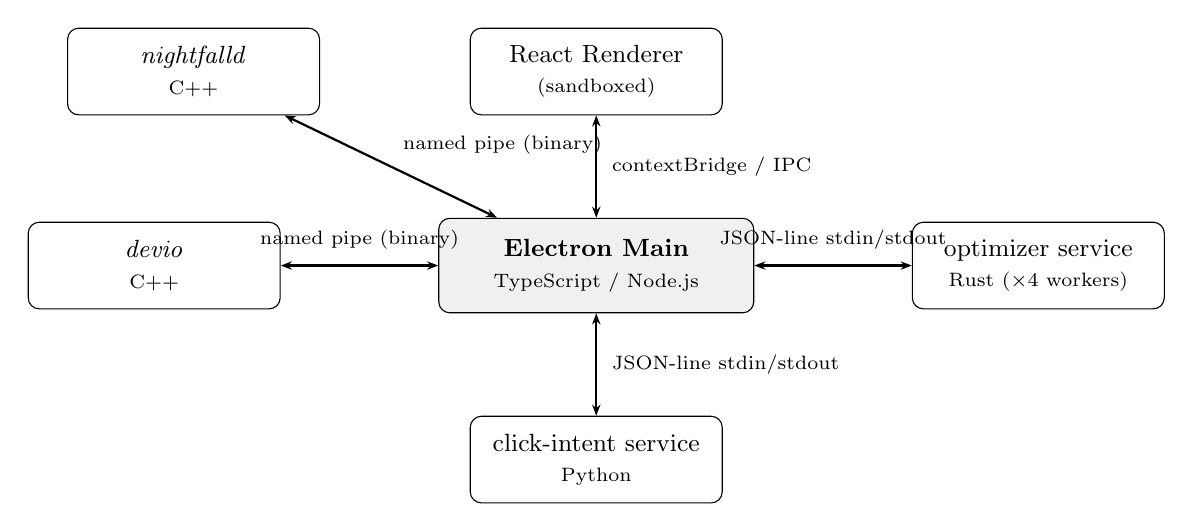
\begin{tikzpicture}[
    font=\small,
    proc/.style={draw, rounded corners=4pt, minimum width=3.2cm, minimum height=1.1cm,
                 align=center, fill=white},
    central/.style={draw, rounded corners=4pt, minimum width=4.0cm, minimum height=1.2cm,
                    align=center, fill=gray!12},
    arr/.style={{Stealth[length=4pt]}-{Stealth[length=4pt]}, thick},
    node distance=1.6cm,
  ]
    % Central hub
    \node[central] (electron)
        {\textbf{Electron Main}\\{\scriptsize TypeScript / Node.js}};

    % React renderer (top)
    \node[proc, above=1.3cm of electron] (react)
        {React Renderer\\{\scriptsize (sandboxed)}};

    % C++ daemons (left)
    \node[proc, left=2.0cm of electron] (devio)
        {\textit{devio}\\{\scriptsize C++}};
    \node[proc, above left=1.3cm and 1.5cm of electron] (nightfall)
        {\textit{nightfalld}\\{\scriptsize C++}};

    % Python service (bottom)
    \node[proc, below=1.3cm of electron] (python)
        {click-intent service\\{\scriptsize Python}};

    % Rust optimizer (right)
    \node[proc, right=2.0cm of electron] (rust)
        {optimizer service\\{\scriptsize Rust ($\times$4 workers)}};

    % Edges with protocol labels
    \draw[arr] (react)    -- node[right=2pt, font=\scriptsize]       {contextBridge / IPC}       (electron);
    \draw[arr] (nightfall)-- node[above right=1pt, font=\scriptsize] {named pipe (binary)}       (electron);
    \draw[arr] (devio)    -- node[above=2pt, font=\scriptsize]       {named pipe (binary)}       (electron);
    \draw[arr] (python)   -- node[right=2pt, font=\scriptsize]       {JSON-line stdin/stdout}    (electron);
    \draw[arr] (rust)     -- node[above=2pt, font=\scriptsize]       {JSON-line stdin/stdout}    (electron);
  \end{tikzpicture}
  \caption{Five-process topology. Arrows denote bidirectional IPC. Rust optimizer uses four concurrent workers; Python service is a persistent daemon.}
  \label{fig:topology}
\end{figure}

\begin{itemize}
    \item \textbf{Host application (TypeScript / Electron):} the main process owns the session store, orchestrates subprocess lifecycle via \texttt{ServerManager}, and exposes a typed IPC bridge to the React renderer. The full signal-processing pipeline runs here as a TypeScript module.
    \item \textbf{Device I/O daemon (\texttt{nightfalld}, C++):} captures HID frames at up to 8,000\,Hz, performs real-time kinematic analysis (trajectory, jitter, click classification), and streams processed events to the host over a named pipe.
    \item \textbf{Device control daemon (\texttt{devio}, C++):} negotiates HID++ feature pages (Analog Buttons 0x1B0C, Analog Keys 0x1B08, DPI 0x2201/0x2202) and writes configuration commands to the peripheral.
    \item \textbf{Click-intent service (Python):} a persistent subprocess that trains and serves the click-intent ML models, receiving commands and emitting progress events over a JSON-line stdin/stdout channel.
    \item \textbf{Optimizer service (Rust):} simulates the RT firmware state machine on recorded telemetry and sweeps the $(AL, RT)$ parameter space, communicating via the same JSON-line protocol.
\end{itemize}

\section{Signal Processing Pipeline}
\label{sec:impl-signal}

\subsection{Data Types and Precision Budget}

All signal buffers use typed arrays. Intermediate computations—Akima spline fitting, Savitzky-Golay coefficient application, analytic second-derivative evaluation—operate on \texttt{Float64Array} (double precision) to prevent rounding-error accumulation across three successive differentiation steps. Results are downcast to \texttt{Float32Array} before storage and downstream consumption, halving memory bandwidth at the cost of approximately $10^{-7}$ relative error, which is negligible relative to the quantization error of the 7-bit step120 signal. Raw step120 integers are promoted to \texttt{Float64Array} at the pipeline entry point and never converted back until the final downcast.

\subsection{Pipeline Entry Point}

\texttt{computeDerivedSignals(step120, settings)} is the single public entry point for all derived channels. It returns a \texttt{DerivedChannel} record containing \texttt{Float32Array} buffers for depth, speed, acceleration, jerk, and drift, plus the interpolation factor in effect (needed by downstream code to convert sub-frame latency shifts). All intermediate allocations are local to this call; no global signal state is retained between invocations.

\subsection{Depth Clamping After Interpolation}

After Makima upsampling, depth is clamped to the physical range $[0, 120]$ step120 units before any smoothing or differentiation step. This is not a guard clause—it is a correctness requirement. Cubic-family interpolants overshoot on abrupt quantization steps: production recordings have shown overshoot to $-21$ step120 ($-0.7$\,mm below the resting surface) and Runge-phenomenon spikes to $+143$ step120 ($+0.77$\,mm past the bottom stop). The Rust optimizer's state machine compares normalised depth against threshold parameters in $[0.0, 1.0]$; unclamped values outside $[0, 120]$ produce make or break events at frames where no actuation occurred, corrupting the entire sweep result silently.

\subsection{Contact-Bounce Blind Window}

When contact-bounce suppression is enabled, the $W_b$-frame masked region is filled by evaluating a natural cubic spline fitted to $W_c$ context frames bracketing the gap. The spline second-derivative vector is computed via the Thomas algorithm—a specialised $O(W_c)$ tridiagonal solver that exploits the strict diagonal dominance of the natural-boundary condition system, avoiding the $O(W_c^2)$ cost of general Gaussian elimination. Each masked frame is then evaluated by the piecewise Hermite formula from its two bracketing knots and their precomputed second derivatives, recovering a smooth trajectory through the bounce window.

\subsection{Peak Mipmap}

Waveform visualisation during session review requires fast range-max queries: the Y-axis scale must be recomputed on every scroll and zoom event. A \texttt{PeakMipmap} is built once per signal in $O(N)$ time as a power-of-two cascade of \texttt{Float32Array} levels, each storing the maximum absolute value over non-overlapping pairs from the level below. A range-max query for $[l, r]$ selects the coarsest level whose cell width is $\leq 64$ samples and traverses the covered cells—a constant number of memory accesses for any fixed display resolution. Without this structure, each scroll event over a 300,000-sample session would require a full $O(N)$ linear scan.

\section{Inter-Process Communication}

\subsection{Named Pipes for C++ Daemons}

\texttt{nightfalld} and \texttt{devio} communicate via platform-native named pipes on Windows and Unix domain sockets on Linux. Pipe names are unique per-process instance: \texttt{gsense\_nightfalld\_\{pid\}\_\{timestamp\}} and \texttt{gsense\_devio\_\{pid\}\_\{timestamp\}}. Uniqueness prevents collision when multiple application windows run simultaneously, and the absence of a well-known port avoids firewall conflicts on restricted networks.

\texttt{devio} is spawned first and given a one-second head-start; \texttt{nightfalld} then receives the devio pipe name as a startup argument. This enforces a unidirectional dependency without a shared global registry: \texttt{nightfalld} can query device capabilities from \texttt{devio} at any point after startup without requiring a service-discovery step.

\subsection{JSON-Line Protocol for Python and Rust}

The click-intent service and optimizer service both use newline-delimited JSON over stdin/stdout. This protocol requires no port allocation, works identically on all platforms, and is natively line-buffered by the OS. Streaming events (training-progress updates, optimizer progress ticks) are emitted as individual lines, so the host receives them incrementally without waiting for the full job to complete. Each command carries a \texttt{job\_id} field; all responses echo the same \texttt{job\_id}, enabling the host to demultiplex concurrent jobs running in separate threads within a single daemon process.

\subsection{ServerManager Orchestration}

\texttt{ServerManager} in the Electron main process owns the lifecycle of all five subprocesses:

\begin{itemize}
    \item \textbf{Heartbeat monitoring.} \texttt{nightfalld} is polled every 10\,s with a 3\,s timeout. Three consecutive failures emit a \texttt{backend-unresponsive} event to the UI and trigger a restart sequence.
    \item \textbf{Auto-restart.} An unexpected exit (code $\neq 0$, signal $\notin \{\text{SIGTERM, SIGKILL}\}$) triggers automatic restart, up to three attempts. Deliberate shutdowns skip this logic.
    \item \textbf{Graceful shutdown.} SIGTERM is issued first; if the process has not exited within 3\,s, SIGKILL follows.
    \item \textbf{Device config restoration.} On USB reconnect or system resume, per-device configurations (DPI, actuation thresholds) are restored. Stored values are percentage-normalised; on reconnect, \texttt{devio} reports the device's current capability range and the manager converts percentages to absolute step values before re-issuing configuration commands.
\end{itemize}

\subsection{Renderer Security Boundary}

The React renderer runs in a sandboxed Electron context and communicates with the main process exclusively through a typed \texttt{contextBridge} preload API. The renderer cannot spawn processes, open named pipes, or access the filesystem directly. This boundary ensures that a malformed session file parsed in the renderer cannot escalate to arbitrary process execution on the host.

\section{RT State Machine Simulation}

The Rust optimizer service is centred on \texttt{state\_machine.rs}, which implements a frame-by-frame simulation of the peripheral firmware's Rapid Trigger FSM. The simulation is the single source of truth for the firmware's behaviour on a given depth trace: the RT state machine is non-differentiable and history-dependent, so there is no closed-form expression for its output as a function of $(AL, RT)$ parameters. The only correct approach is to simulate it frame-by-frame on the actual recorded data.

\paragraph{Non-RT mode (2-state FSM).}
\begin{itemize}
    \item \textbf{IDLE:} $\mathrm{signal}[t] \geq \theta_\mathrm{make}$ $\Rightarrow$ emit make event, transition to \textbf{PRESSED}.
    \item \textbf{PRESSED:} $\mathrm{signal}[t] \leq \theta_\mathrm{break}$ $\Rightarrow$ emit break event, transition to \textbf{IDLE}.
\end{itemize}

\paragraph{RT mode (3-state hysteresis FSM).}
\begin{itemize}
    \item \textbf{IDLE:} $\mathrm{signal}[t] \geq \theta_\mathrm{make}$ $\Rightarrow$ emit make event, set $\mathrm{peak} \leftarrow \mathrm{signal}[t]$, transition to \textbf{PRESSED}.
    \item \textbf{PRESSED:} update $\mathrm{peak} \leftarrow \max(\mathrm{peak},\, \mathrm{signal}[t])$. If $\mathrm{signal}[t] \leq \mathrm{peak} - \Delta_\mathrm{RT}$ $\Rightarrow$ emit break event, set $\mathrm{valley} \leftarrow \mathrm{signal}[t]$, transition to \textbf{RT\_RELEASED}.
    \item \textbf{RT\_RELEASED:} update $\mathrm{valley} \leftarrow \min(\mathrm{valley},\, \mathrm{signal}[t])$. If $\mathrm{signal}[t] \leq 0$ $\Rightarrow$ reset to \textbf{IDLE}. If $\mathrm{signal}[t] \geq \mathrm{valley} + \Delta_\mathrm{RT}$ $\Rightarrow$ emit make event, transition to \textbf{PRESSED}.
\end{itemize}

\paragraph{Parallel sweep.}
Four input signals (depth, speed, acceleration, jerk) are crossed with two threshold types (make and break thresholds independently), yielding 16 distinct (signal, threshold) combinations. Each combination is evaluated independently using Rayon's work-stealing thread pool, which allocates $n_\mathrm{CPUs} - 2$ threads to leave cores available for the Electron main process and C++ daemons. The full evaluated grid and Pareto frontier are serialised to a per-run JSON sidecar alongside the in-memory result, enabling post-hoc inspection of the complete loss landscape without re-running the sweep.

\section{ML Service: Training Pipeline and Model Lifecycle}

\subsection{Daemon Architecture}

The click-intent service runs as a persistent Python subprocess. The main thread blocks on \texttt{stdin.readline()}, dispatching each command to a new worker thread. A per-job \texttt{threading.Event} cancel flag is checked at epoch boundaries, enabling clean mid-epoch termination without corrupting in-progress checkpoints. All \texttt{stdout} writes are serialised by a global \texttt{threading.Lock}, preventing line interleaving from concurrent progress events across simultaneous jobs.

\subsection{Model Persistence and Reproducibility}

Each trained model occupies its own directory containing:
\begin{itemize}
    \item \texttt{config.json} — architecture hyperparameters and training configuration
    \item \texttt{weights.pkl} / \texttt{.pt} — serialised weights (joblib for scikit-learn models, \texttt{torch.save} for the FCN)
    \item \texttt{metrics.json} — per-class validation F1, confusion matrix, and inference benchmark
    \item \texttt{info.json} — provenance metadata including an SHA-256 input fingerprint
    \item \texttt{resume.json} + \texttt{checkpoints/} — present only during a paused training run
\end{itemize}

The model ID follows the convention \texttt{\{arch\}\_\{channel\}\_\{param\_hash\}\_\{timestamp\}}, where \texttt{param\_hash} is an 8-character prefix of the SHA-256 digest of the full training configuration. Two identical configurations on the same data produce the same hash, enabling cache hits and reproducible ablation comparisons without manual bookkeeping. After training, the model is profiled on 2,000 frames across three warm-up trials; the minimum observed latency is recorded as \texttt{ms\_per\_frame} in \texttt{metrics.json}, providing an immediate deployment-readiness indicator.

\subsection{Data Augmentation}

Two augmentation strategies are applied at training time only, never to the held-out validation or test partitions.

\textbf{Channel flip.} Left (L) and right (R) analog channels are swapped, treating the left-button recording as a right-button recording and vice versa. All preprocessing parameters that refer to a specific side (actuation thresholds, hysteresis values) are mirrored correspondingly. This doubles the effective training set at zero annotation cost, exploiting the bilateral symmetry of the click task.

\textbf{Noise and smoothing perturbation.} Gaussian noise (with $\sigma$ sampled per augmented copy) is injected into the normalised depth signal after preprocessing, and the smoothing window is perturbed within a small neighbourhood of its nominal value. Smoothing perturbation is memoized via an LRU cache keyed on window size, amortising the cost of Akima re-computation when the same window appears across multiple augmented copies of the same session.

\subsection{Batch Inference and Overlap Handling}

Full-session prediction is split into 30,000-frame chunks. The fixed dispatch overhead of scikit-learn's \texttt{predict\_proba} (${\approx}14$\,ms per call, independent of chunk size) makes very small chunks wasteful; 30,000 frames keeps the overhead below 0.05\,\% of total inference time while fitting within cache. Adjacent chunks overlap by the classifier's temporal receptive field—32\,frames for RF and GBT, 3,060 frames for the OfflineFCN. After all chunks are predicted, the left half of each overlapping region is taken from the left chunk and the right half from the right chunk, eliminating boundary artefacts without requiring additional smoothing of the probability output.

Optuna hyperparameter-sweep studies are persisted to a per-session SQLite file. On application restart, incomplete sweeps resume from the last completed trial without re-evaluating previously explored configurations.


%%%%%%%%%%%%%%%%%%%%
\chapter{Evaluation}
\label{chap:eval}
%%%%%%%%%%%%%%%%%%%%

This chapter evaluates the three core contributions of the system: (1) the programmatic labeling pipeline and the quality of the resulting click-intent annotations; (2) the four-class temporal sequence classifier, measured by per-class F1 across models and ablation conditions; and (3) the joint AL/RT optimizer, measured by latency reduction and false-positive suppression relative to default factory settings.

\section{Evaluation Setup}

\subsection{Dataset}

The evaluation dataset consists of recorded sessions collected under two conditions:

\begin{itemize}
    \item \textbf{Personal recordings} from users, stored in \texttt{data/recordings/}.
          Each session is a 3--10 minute unstructured gaming segment recorded at 1\,kHz
          from a Logitech SUPERSTRIKE or Hall-effect keyboard device with analog depth
          firmware enabled.
    \item \textbf{External benchmark recordings} from \texttt{data/external\_ab\_data/}:
          32 recordings collected from external users under an A/B comparison protocol
          (default vs.\ optimised settings), each approximately 5 minutes at 1\,kHz.
\end{itemize}

Across all sessions, the dataset contains approximately [N\_total] click events, with a mean of [N\_clicks] clicks per session at a median press duration of [D\_make]\,ms (make onset), [D\_hold]\,ms (hold), and [D\_break]\,ms (break onset).

\subsection{Metrics}

\paragraph{Classifier.}
Per-class F1 score for each of the four target classes (\texttt{BG}, \texttt{MAKE\_ONSET}, \texttt{CLICK\_HOLD}, \texttt{BREAK\_ONSET}) and macro-F1 averaged across the three non-background classes. All thresholds use the default $\theta_m = \theta_b = 0.02$. A confusion matrix is reported at the same threshold.

\paragraph{Optimizer.}
Mean actuation latency (ms), false-positive rate (spurious make events per 100 click events), and click recall (fraction of labeled click events recovered by the simulated firmware). Metrics are reported before and after optimization, relative to the default factory settings (AL = 2.0\,mm, RT = 0.2\,mm).

\subsection{Baselines}
\label{sec:baselines}

\paragraph{Geometric auto-labeler baseline.}
The geometric auto-labeler's own label assignments are used as predictions on the held-out frames. Because the classifier is trained on these same labels, this baseline measures self-consistency---how well the model reproduces the heuristic it was trained on---rather than absolute click-intent detection accuracy.

This is an important validity constraint: the absolute F1 numbers, when available, will quantify label fidelity to the heuristic, not ground-truth click-intent accuracy. A classifier that exactly reproduces the auto-labeler would score perfect F1 against this baseline despite having learned nothing beyond the heuristic. The relative comparison between models (RF vs.\ GBT vs.\ FCN) remains internally valid because all models are evaluated against the same labels; however, absolute F1 numbers cannot be interpreted as accuracy without an independent reference. The primary defensible claim of the classifier is therefore not its absolute F1, but its downstream effect on the optimizer: if the ML classifier produces better-quality click annotations than the auto-labeler alone, the optimizer should find lower-loss configurations, which is measured directly in Section~\ref{sec:optimizer-results}.

\paragraph{Velocity-threshold baseline.}
A fixed velocity-threshold rule is used as a second classifier baseline that does not share the auto-labeler's label distribution: a frame is predicted as \texttt{MAKE\_ONSET} if the centered velocity $v[t] < -h_m$ (finger descending faster than threshold $h_m$) and as \texttt{BREAK\_ONSET} if $v[t] > +h_b$; all remaining frames are predicted as \texttt{BG} or \texttt{CLICK\_HOLD} based on depth level. Thresholds $h_m$ and $h_b$ are selected by grid search on the training partition. This baseline shows whether the ML classifier provides value beyond a naive rule applied to the raw signal, independent of the label-quality question. A classifier that fails to outperform this velocity rule on held-out sessions provides weak evidence for the learned features.

\paragraph{Optimizer baseline.}
Default factory settings (AL = 2.0\,mm, RT = 0.2\,mm), the manufacturer defaults shipped with each device, are used as the reference for all optimizer metrics.

\subsection{Train/Validation Split}

All sessions are split by click boundary: the first 80\% of click events (in temporal order) form the training partition and the remaining 20\% form the held-out validation partition. This temporal split prevents receptive-field leakage: a model with a 3,060-frame ($\pm$1530\,ms) receptive field that trained on a random 80\% sample drawn from the full session would have, in expectation, training context overlapping with every validation frame. The click-boundary split ensures that no training frame lies within the receptive field of any validation frame.

\section{Click-Intent Classifier Results}

Table~\ref{tab:classifier} reports per-class F1 for all four models averaged over the held-out validation partitions across all sessions.

\begin{table}[t]
\centering
\begin{tabular}{l*{4}{r}}
\toprule
Model & Make & Hold & Break & Macro \\
\midrule
Velocity rule & --- & --- & --- & --- \\
Auto-labeler  & --- & --- & --- & --- \\
\midrule
RF       & --- & --- & --- & --- \\
GBT    & --- & --- & --- & --- \\
FCN          & --- & --- & --- & --- \\
CRF+FCN           & --- & --- & --- & --- \\
\bottomrule
\end{tabular}
\caption{Per-class F1 on validation partitions. Auto-labeler measures self-consistency; dashes indicate pending experimental completion.}
\label{tab:classifier}
\end{table}

Three qualitative predictions follow from the design:

\begin{itemize}
    \item \textbf{GBT $>$ RF on MAKE\_ONSET.} GBT trains end-to-end on the
          asymmetric soft-label loss via a custom differentiable objective; RF converts soft
          targets to hard labels before tree-fitting, discarding the distributional information
          in the soft targets. This should manifest as higher make-onset F1 for GBT,
          particularly at short sessions where the calibration of each boundary frame matters.

    \item \textbf{OfflineFCN $>$ shallow models on long-context clicks.} The
          OfflineFCN's $\pm$1530\,ms receptive field can observe the slow pre-press
          approach ramp hundreds of milliseconds before actuation---a cue inaccessible to
          the 32\,ms shallow window. This advantage is most pronounced for users with
          slow deliberate press velocities, where the intent signal accumulates over
          hundreds of milliseconds.

    \item \textbf{CRF $>$ OfflineFCN on BREAK\_ONSET precision.} The CRF transition
          matrix penalizes physically impossible sequences (e.g.\ isolated
          \texttt{BREAK\_ONSET} without a preceding \texttt{MAKE\_ONSET} run). This
          should reduce false-positive break detections and improve precision on
          \texttt{BREAK\_ONSET} relative to per-frame argmax decoding.
\end{itemize}

\section{Ablation Studies}

Three ablations isolate the contribution of specific design choices.

\subsection{Soft-Label Parameterization}

To measure the impact of the asymmetric soft-label training target, three conditions are compared on the GBT model:

\begin{enumerate}
    \item \textbf{Hard labels:} the auto-labeler's boundary frames are used as hard
          one-hot targets.
    \item \textbf{Symmetric Gaussian:} a single $\sigma = 5$ frames is applied on
          both sides of each boundary.
    \item \textbf{Asymmetric Gaussian:} separate $\sigma_\mathrm{left}$ and
          $\sigma_\mathrm{right}$ for \texttt{MAKE\_ONSET} and \texttt{BREAK\_ONSET},
          as described in Section~\ref{sec:training}.
\end{enumerate}

The expected ordering is: asymmetric $>$ symmetric $>$ hard, with the largest gap on \texttt{MAKE\_ONSET} F1. Make onsets are physically sharper than break onsets: the backward search labeling function introduces wider timing uncertainty on the pre-press side (where the search may stop early at a plateau) than on the post-actuation side (where the downward motion is already confirmed by the hardware event). The asymmetric Gaussian encodes this asymmetry; a symmetric Gaussian over-smooths the sharp post-actuation side, degrading precision.

\begin{table}[t]
\centering
\begin{tabular}{lrr}
\toprule
Training target & MAKE\_ONSET F1 & Macro-F1 \\
\midrule
Hard labels         & ---  & ---  \\
Symmetric Gaussian  & ---  & ---  \\
Asymmetric Gaussian & ---  & ---  \\
\bottomrule
\end{tabular}
\caption{Ablation: soft-label parameterization on GBT. Dashes indicate results pending.}
\label{tab:ablation_softlabel}
\end{table}

\subsection{Auto-Labeler Sensitivity}

To measure how sensitive the ML classifier is to auto-labeler quality, the plateau patience parameter $p$ is varied from 5 to 30 frames while holding all other parameters fixed. Smaller $p$ causes earlier termination of the backward search, systematically labeling \texttt{MAKE\_ONSET} frames too late relative to true intent; larger $p$ risks including plateau frames where no pressing motion is occurring.

The expected relationship is non-monotone: performance degrades sharply at $p < 8$ (onset labels too late, missing the genuine press onset) and degrades more gradually at $p > 20$ (onset labels too early, into the plateau region). The default $p = 15$ targets the center of this range, covering the typical pre-press deceleration phase without extending into the flat resting region.

\subsection{Per-Session vs.\ Cross-User Generalization}

To quantify the value of per-session retraining, a cross-user evaluation is conducted:

\begin{enumerate}
    \item \textbf{Per-session:} model trained on clicks 1--80\% of a session from
          user $X$, evaluated on clicks 80--100\% of the same session.
    \item \textbf{Cross-user:} model trained on all sessions from user $X$, evaluated
          on sessions from a different user $Y$.
\end{enumerate}

A substantial macro-F1 drop in the cross-user condition would confirm the per-session retraining design choice. The magnitude of this drop quantifies the fraction of classification performance attributable to idiosyncratic user-specific features---resting depth, press velocity, release curvature---that a cross-user model cannot capture. Cross-user transfer is expected to perform worse than per-user but above the geometric baseline, since the global model at minimum learns the general temporal structure of click-intent boundaries shared across users.

\section{Parameter Optimizer Results}
\label{sec:optimizer-results}

For each evaluated session, the optimizer reports the Pareto frontier in the recall--mean latency plane before and after optimization. Table~\ref{tab:optimizer} summarises the aggregate results.

\begin{table}[t]
\centering
\begin{tabular}{lrrr}
\toprule
Condition & Mean latency (ms) & FP rate (/100 events) & Recall \\
\midrule
Default (AL=2.0\,mm, RT=0.2\,mm) & ---  & ---  & ---  \\
Grid search ($50{\times}50$)      & ---  & ---  & ---  \\
Joint CMA-ES                      & ---  & ---  & ---  \\
\midrule
$\Delta$ (CMA-ES vs.\ default)   & ---  & ---  & ---  \\
\bottomrule
\end{tabular}
\caption{Optimizer results averaged across all evaluated sessions. Grid search over a
  $50{\times}50$ AL/RT grid is included as a baseline to verify that CMA-ES finds
  equivalent configurations. Dashes indicate results pending.}
\label{tab:optimizer}
\end{table}

The Pareto frontier---a scatter plot in the recall--latency plane with one point per evaluated (AL, RT) candidate and the Pareto-optimal subset highlighted---is the primary output of the optimizer. The key qualitative expectation is that the joint CMA-ES sweep identifies configurations that strictly dominate the default factory settings in at least one objective: lower latency at equivalent false-positive rate, or lower false-positive rate at equivalent latency.

The optimizer's advantage over the default configuration is expected to be largest for users who exhibit a low-velocity press style (where a lower AL is safe) or users whose resting depth sits close to the factory AL (where RT sensitivity must be raised to avoid accidental make events from resting-weight drift). For users whose factory defaults happen to match their biomechanics, the optimizer should reproduce the default configuration rather than diverging from it, confirming that the search converges correctly.

\subsection{Loss Weight Sensitivity Analysis}
\label{sec:lambda-sensitivity}

To assess the robustness of the recommended configuration to the arbitrary penalty weights in Equation~\ref{eq:loss}, the optimizer is re-run with $\lambda_\mathrm{miss}$ and $\lambda_\mathrm{false}$ each varied by $\pm$50\% independently, yielding a $3 \times 3 = 9$-point sensitivity grid. Table~\ref{tab:lambda-sensitivity} reports the resulting recommended (AL, RT) configurations and their objective values.

\begin{table}[t]
\centering
\begin{tabular}{rrrrr}
\toprule
$\lambda_\mathrm{miss}$ & $\lambda_\mathrm{false}$ & Rec.\ AL (mm) & Rec.\ RT (mm) & $\Delta$latency (ms) \\
\midrule
5  & 2.5 & --- & --- & --- \\
5  & 5.0 & --- & --- & --- \\
5  & 7.5 & --- & --- & --- \\
10 & 2.5 & --- & --- & --- \\
10 & 5.0 & --- & --- & --- \\
10 & 7.5 & --- & --- & --- \\
15 & 2.5 & --- & --- & --- \\
15 & 5.0 & --- & --- & --- \\
15 & 7.5 & --- & --- & --- \\
\bottomrule
\end{tabular}
\caption{Sensitivity of recommended (AL, RT) to $\pm$50\% perturbation of the default loss weights. Small variation across cells indicates robust recommendations; large variation indicates the result depends on the specific weight calibration.}
\label{tab:lambda-sensitivity}
\end{table}

\section{Discussion}

\subsection{Strengths of the Proposed Approach}

The programmatic labeling pipeline eliminates the annotation bottleneck that has historically prevented supervised learning on HID telemetry at millisecond resolution. Because annotations are derived automatically from the hardware click event stream and the depth signal geometry, the system can scale to any number of recordings without additional labeling cost. The asymmetric soft-label correction partially absorbs the heuristic's timing errors, and the per-session retraining ensures that each user's model reflects their own control signature rather than a population average.

The joint CMA-ES optimizer addresses a practical limitation of all prior RT/AL tuning approaches: the two parameters interact. A low AL reduces pre-travel latency but increases the risk of accidental actuation from resting finger weight; a high RT sensitivity eliminates the fixed reset point but creates accidental double-clicks if resting noise exceeds the RT threshold. The joint optimizer explicitly models this interaction by simulating the firmware on the user's own recorded telemetry, producing recommendations that are grounded in the user's actual click dynamics rather than generic guidelines.

\subsection{Limitations of the Evaluation}

\paragraph{Circular evaluation — a validity threat, not a caveat.}
The classifier is trained on labels generated by the geometric auto-labeler. The primary classifier baseline is also the geometric auto-labeler used as a predictor. The absolute F1 numbers therefore measure label fidelity to the heuristic, not click-intent detection accuracy against ground truth. This is a structural validity threat: a model that perfectly reproduces the heuristic would score 1.0 F1 in this evaluation without having learned anything useful.

The threat is partially mitigated by two design choices. First, the velocity-threshold baseline (Section~\ref{sec:baselines}) provides a label-independent comparison that does not share the auto-labeler's label distribution; outperforming it is a necessary (though not sufficient) condition for the classifier to be useful. Second, the downstream optimizer outcome---whether the system finds better AL/RT configurations than the default---does not depend on F1 against auto-labels and provides an independent measure of whether the classifier annotations are informative.

A complete resolution would require an independent annotation study: trained annotators marking click-intent boundaries from slow-motion depth signal replays and audio cues. Even 5 annotated sessions would provide an external reference point sufficient to calibrate the auto-labeler's timing bias. This is planned as follow-on work.

\paragraph{On-device path not evaluated.}
The TinyML/on-device inference path described in the Background is not evaluated. Latency and accuracy of an on-device quantized model would require access to the peripheral MCU's development environment and firmware build chain, which were not available within the scope of this project. The on-device evaluation is deferred to future work (Section~\ref{sec:conclusion-fw}).

\paragraph{Session coverage.}
The 32 external benchmark recordings span a range of users and devices but were collected under a structured A/B protocol rather than natural gaming sessions. Protocol-induced behavior---users consciously monitoring their click feel during an A/B test---may not fully represent the unstructured play patterns for which the system is designed. The personal recordings in \texttt{data/recordings/} represent more naturalistic usage but cover fewer users.


%%%%%%%%%%%%%%%%%%%%%%
\chapter{Conclusion}
%%%%%%%%%%%%%%%%%%%%

\section{Summary}

This thesis presented an offline adaptive calibration pipeline for analog peripherals with continuous depth sensing. The work addresses a practical limitation of current firmware: static actuation thresholds that do not adapt to per-user biomechanics, device variability, or within-session fatigue.

The main contributions are:

\begin{itemize}
        \item A \textbf{programmatic labeling pipeline} that derives frame-level
          \texttt{MAKE\_ONSET}, \texttt{CLICK\_HOLD}, and \texttt{BREAK\_ONSET}
            annotations from raw 1\,kHz depth telemetry without manual frame labeling.
            A geometric weak-supervision heuristic is combined with asymmetric soft labels
            to model directional timing uncertainty at boundaries.

        \item A \textbf{four-class temporal sequence classifier} with two model paths. The
          shallow path (Random Forest, Gradient Boosted Trees) operates on hand-crafted
            sliding-window features and supports rapid per-session retraining. The deep path
            (dilated residual FCN with CRF decoding) operates on raw four-channel telemetry
            with a learned $\pm$1530\,ms receptive field, trading higher context for higher
            compute cost.

    \item A \textbf{joint CMA-ES optimizer} that simulates the peripheral firmware's
          Rapid Trigger state machine frame-by-frame and finds Pareto-optimal (AL, RT)
          configurations under latency and false-positive objectives, replacing manual
          threshold sweeps with a data-driven trade-off analysis.
\end{itemize}

In aggregate, these components provide an end-to-end workflow in which a user recording can be automatically labeled, modeled, and optimized to produce evidence-based AL/RT recommendations with minimal manual intervention.

\section{Limitations}
\label{sec:limitations}

Several limitations constrain the generality of the current system:

\begin{itemize}
    \item \textbf{Small evaluation cohort.} The system was evaluated on a limited number
          of users and sessions. Cross-user generalization---whether a model trained on
          one user's data transfers meaningfully to another---was not demonstrated at
          scale. The per-session training approach mitigates this by avoiding cross-user
          transfer entirely, but the cold-start problem for first-time users with no
          prior recordings is not addressed.

    \item \textbf{Auto-labeler timing errors.} The geometric labeling heuristic
          introduces systematic timing bias of up to $W_b$ frames. While asymmetric soft
          labels partially absorb this uncertainty, they do not eliminate it. Make-onset
          F1 is sensitive to the plateau patience parameter, confirming that labeler
          quality is a first-order determinant of classification performance.

    \item \textbf{Offline-only inference.} The OfflineFCN's symmetric non-causal
          padding is incompatible with streaming inference on the peripheral MCU. Any
          deployment on the on-device path would require a causal (left-padded)
          architectural variant, which reduces the per-layer receptive field contribution
          by half.

    \item \textbf{Drift channel unused in the optimizer.} The drift channel
          ($\mathrm{EMA}_{20} - \mathrm{EMA}_{200}$) is computed and exposed in the
          session review UI but is not integrated into the optimizer's objective function.
          As a result, the system does not currently adapt AL/RT recommendations in
          response to detected fatigue-induced resting-weight shift.
\end{itemize}

\section{Future Work}
\label{sec:conclusion-fw}

\begin{enumerate}
    \item \textbf{On-device deployment.} Quantize the OfflineFCN to INT8 and evaluate
          inference latency on the peripheral RISC-V MCU. Develop a causal (left-padded)
          variant compatible with streaming inference. A causal model would convert the
          offline classifier into a real-time intent detector, enabling the pre-report
          filtering described in the Background.

    \item \textbf{Multi-session accumulation.} Train on pooled data from a user's full
          recording history rather than re-training from scratch each session. A
          multi-session model accumulates evidence about the user's long-term
          biomechanical signature, reducing label noise from individual sessions and
          improving performance on edge cases (fatigue-modulated dynamics, device
          warm-up transients).

    \item \textbf{Drift-aware re-calibration.} Integrate the drift channel into the
          optimizer's objective: trigger an automatic re-calibration recommendation when
          sustained positive drift exceeds a per-user threshold, indicating flexor-fatigue
          onset. This closes the loop between the fatigue diagnostic described in
          Section~\ref{sec:drift} and the AL/RT adaptation.

    \item \textbf{Cross-user pre-training.} Pre-train the FCN on pooled data from
          multiple users and fine-tune per-session, reducing the cold-start problem for
          new users with short recording histories. A pre-trained backbone should require
          fewer labeled frames to reach stable performance than a randomly initialized
          model.
\end{enumerate}

\cleardoublepage
\phantomsection
\addcontentsline{toc}{chapter}{Bibliography}
\printbibliography

% Appendices are optional
% \appendix
% %%%%%%%%%%%%%%%%%%%%%%%%%%%%%%%%%%%%%%
% \chapter{How to make a transmogrifier}
% %%%%%%%%%%%%%%%%%%%%%%%%%%%%%%%%%%%%%%
%
% In case you ever need an (optional) appendix.
%
% You need the following items:
% \begin{itemize}
% \item A box
% \item Crayons
% \item A self-aware 5-year old
% \end{itemize}

\end{document}
